%%%%%%%%%%%%%%%%%%%%%%%%%%%%%%%%%%%
% CHAPTER 5: Results + Discussion %
%%%%%%%%%%%%%%%%%%%%%%%%%%%%%%%%%%%
%................................
% Notes about things to add/edit 
%................................
% >> Add plots of gas data stochiometric stuff+
% >> Evaluate comparison of HF and Velocity data and decide if it should be included
% >> Average velocity along entire door?
% >> Flame height via video footage?
% >> Linear plots of parameters vs. each other
%%%%%%%%%%%%%%%%%%%%%%%%%%%%%%%%%%%%%%%%%%%%%%%%%%%%%%%%%%%%%%%%%%%%%
\renewcommand{\thechapter}{5}

\chapter{Results and Discussion}
\label{chap:results_disc}
The figures presented in the following sections compare the predicted quantities output by FDS to the experimental data measured by instrumentation. First, the results of the mesh sensitivity study that was performed to determine an appropriate grid size for the simulations are presented and discussed. Then, the data from the FDS simulations are compared to the sensor data from the nine experiments. Two types of graphs are included with the discussion for each type of measured quantity: one that shows the experimental data and FDS simulation data plotted over the duration of an experiment and a log/log scatter plot of the FDS data vs. the experimental data from all experiments along with some additional statistics to express the accuracy of the FDS models in predicting the specific quantity of interest. All plotted data were time-averaged over 10~seconds in order to smooth the raw data.

\section{Mesh Sensitivity Studies}
\label{sec:mesh_studies}
Figures~\ref{fig:east_O2_sensitivity}--\ref{fig:west_cjet_sensitivity} show the $O_2$ volume fractions and ceiling jet temperatures output by FDS models with coarse, medium, and fine grid sizes for simulations of Tests~4 and 25.
\begin{figure}[!h]
	\centering
	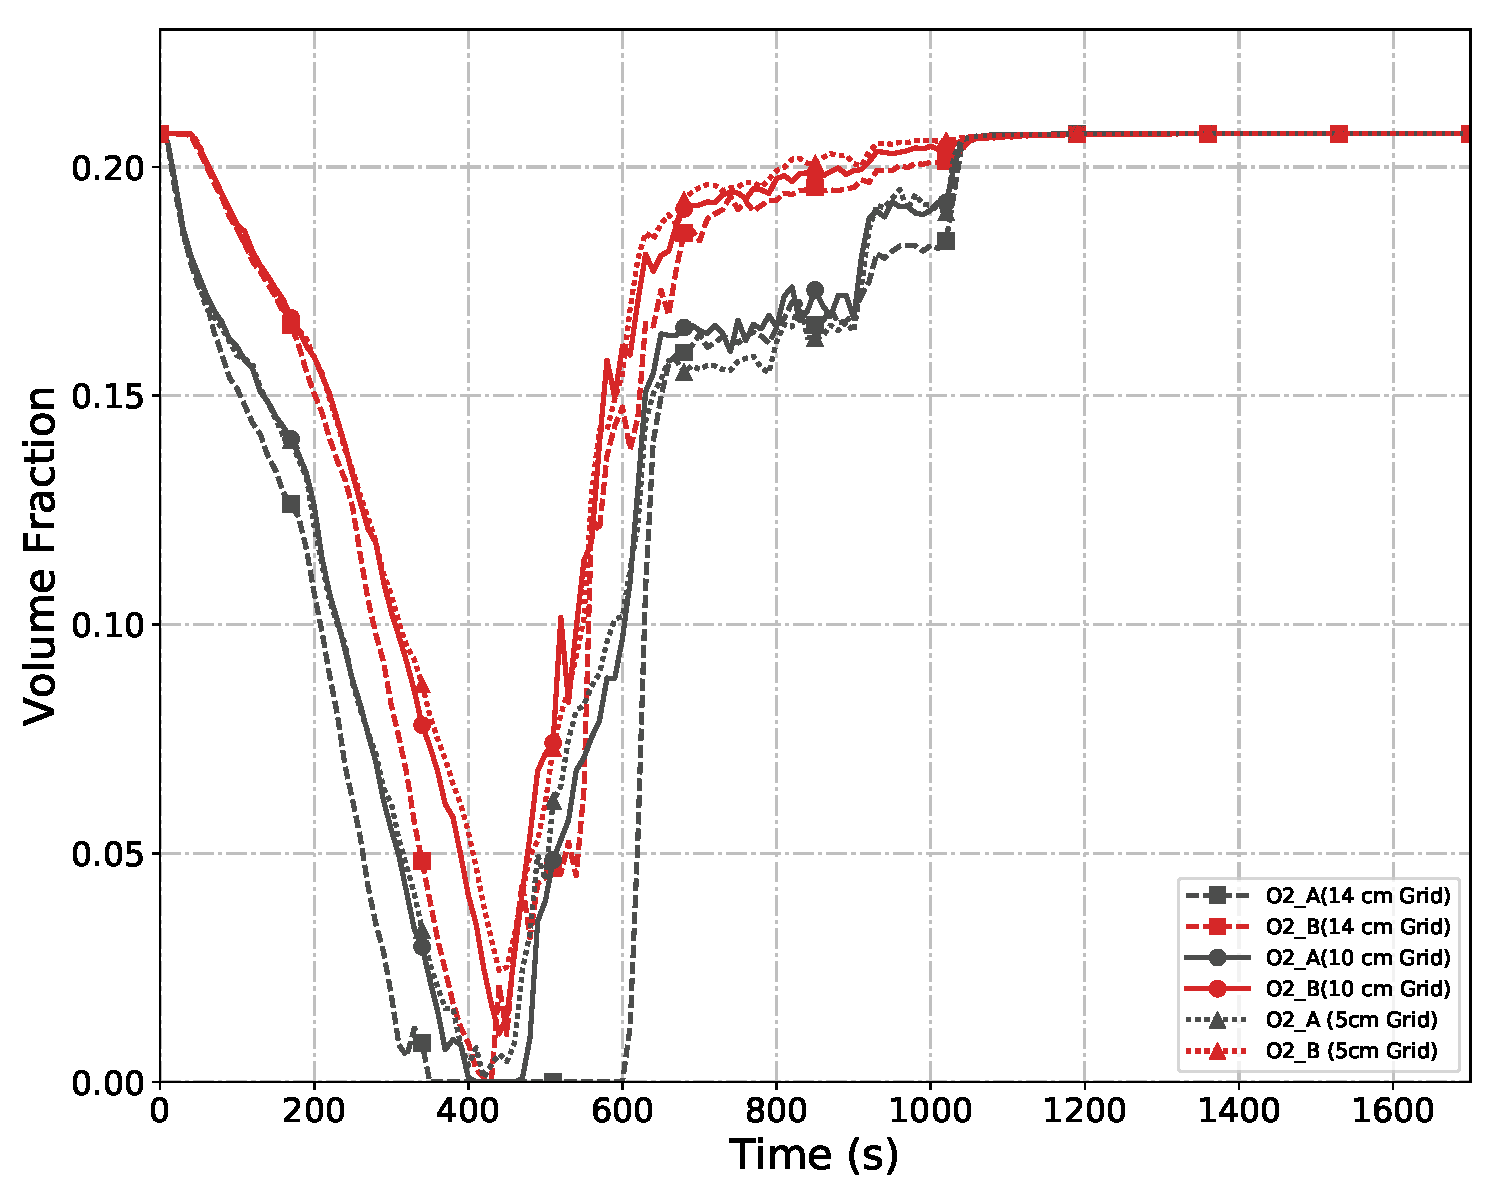
\includegraphics[width=\columnwidth]{../../Plots/Grid_Sensitivity/Gas_Concentration/Test_04_O2}
	\caption[$O_2$ concentrations for East Structure simulations of various mesh sizes.]{$O_2$ concentrations output by the FDS simulations with various mesh sizes for Test~4 in the East Structure.}
	\label{fig:east_O2_sensitivity}
\end{figure}

\begin{figure}[!h]
	\centering
	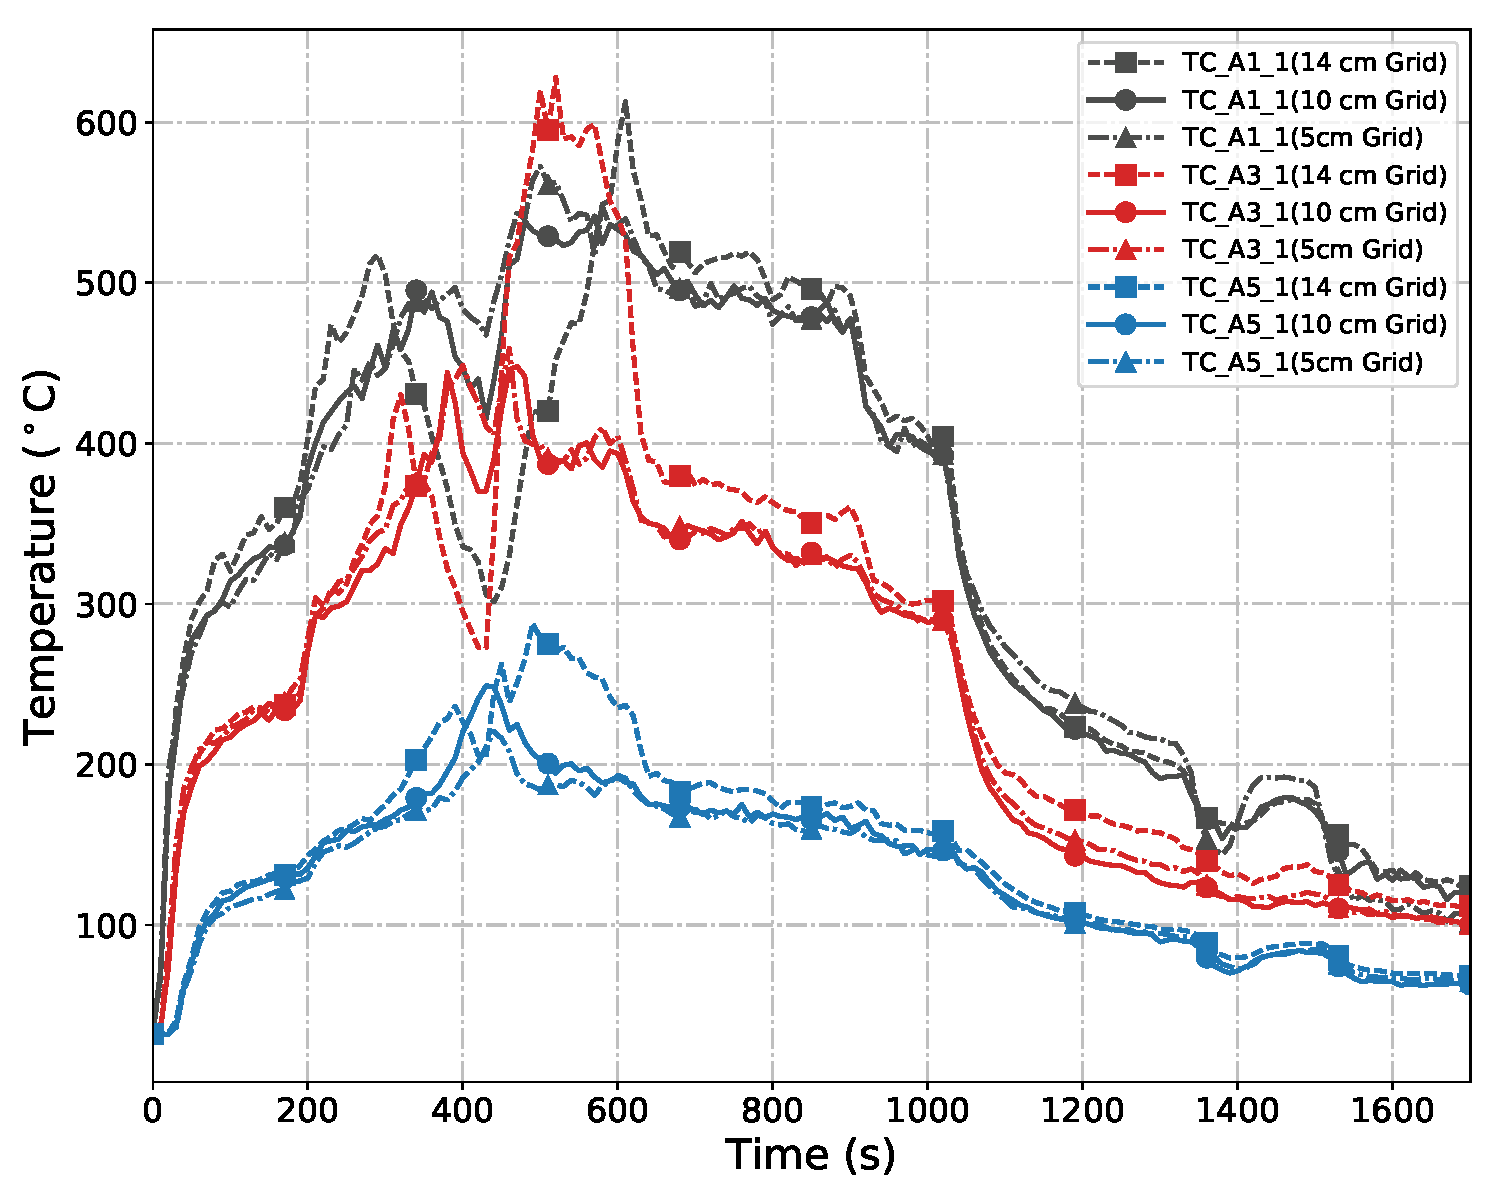
\includegraphics[width=0.87\columnwidth]{../../Plots/Grid_Sensitivity/Temperature/Test_04_cjet_1}
	\\~\\
	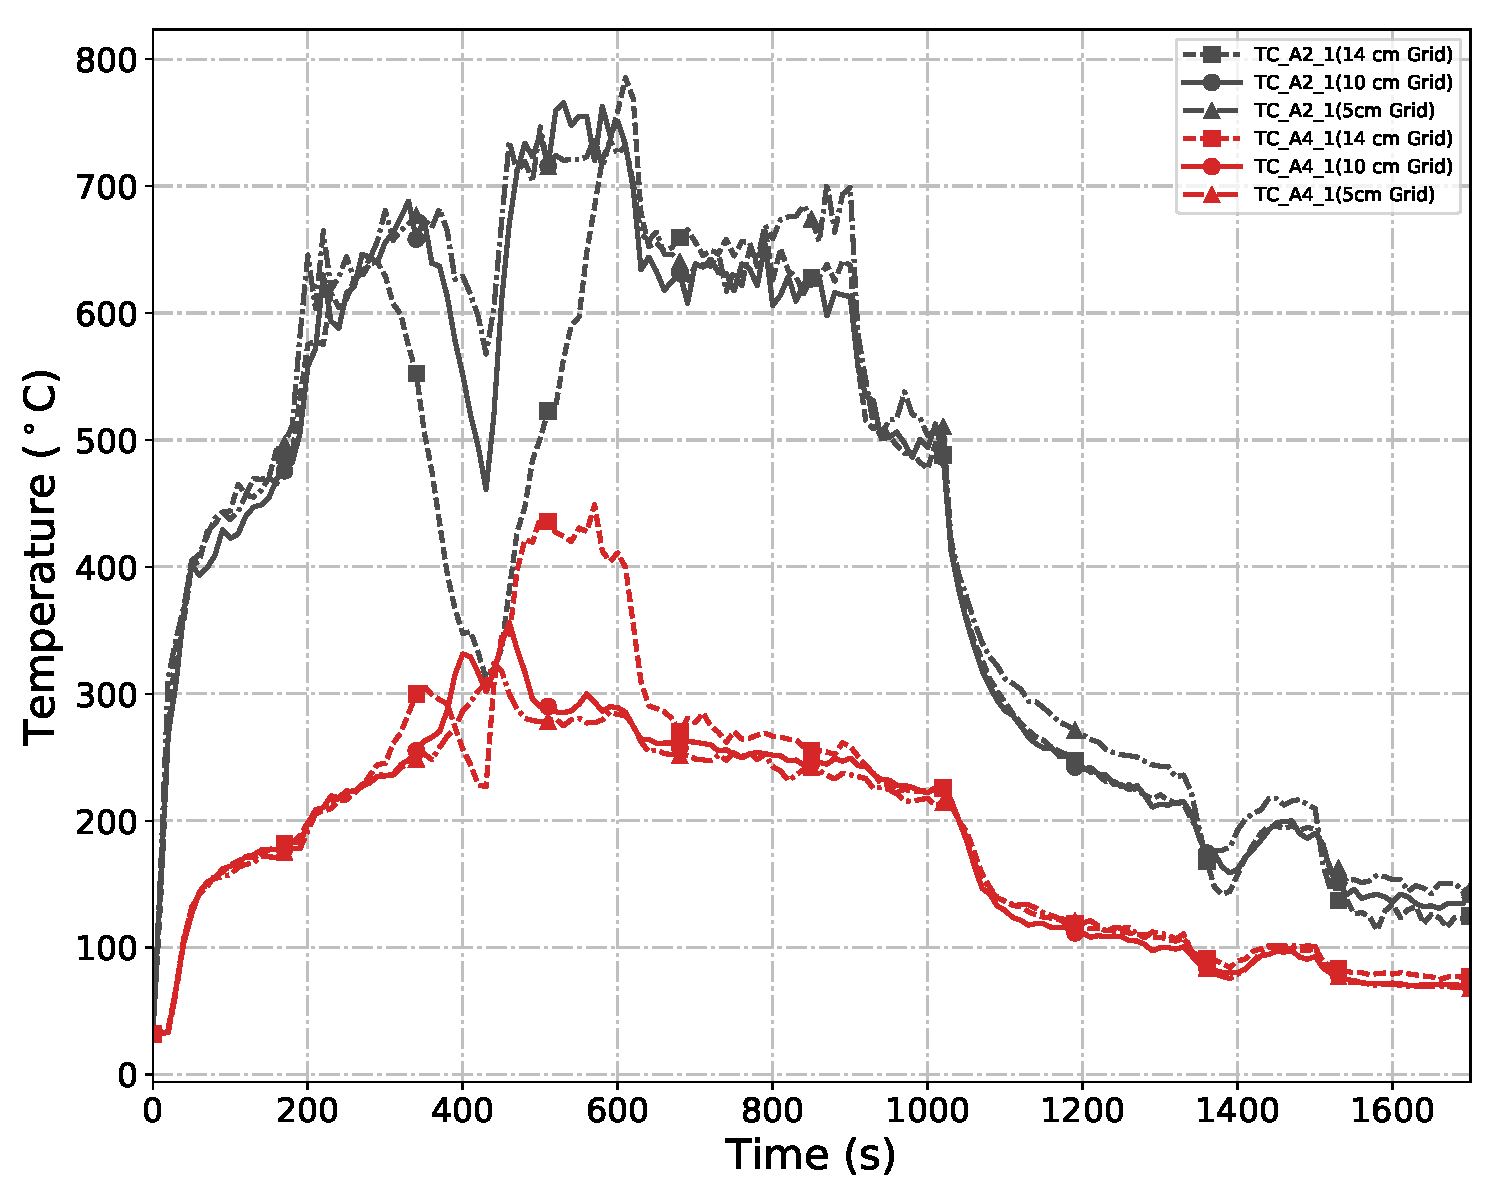
\includegraphics[width=0.87\columnwidth]{../../Plots/Grid_Sensitivity/Temperature/Test_04_cjet_2}
	\caption[Ceiling jet temperatures for East Structure simulations of various mesh sizes.]{Ceiling jet temperatures output by the FDS simulations with various mesh sizes for Test~4 in the East Structure.}
	\label{fig:east_cjet_sensitivity}
\end{figure}

\begin{figure}[!h]
	\centering
	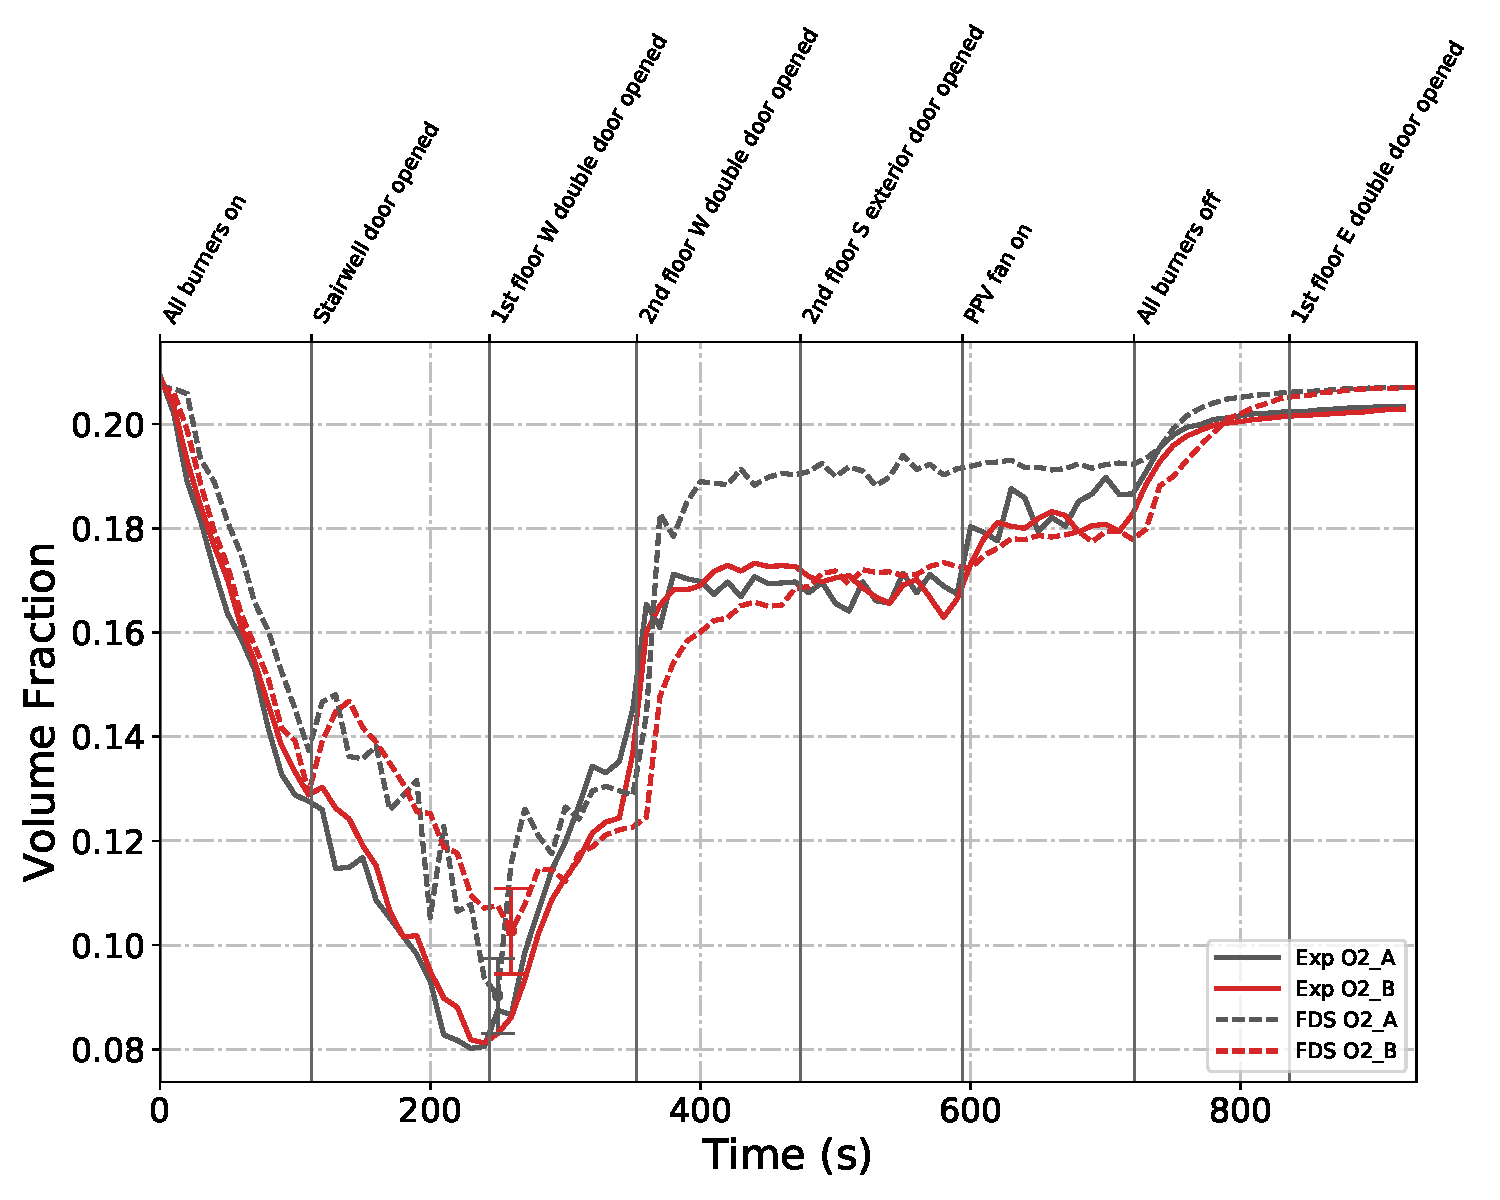
\includegraphics[width=\columnwidth]{../../Plots/Grid_Sensitivity/Gas_Concentration/Test_25_O2}
	\caption[$O_2$ concentrations for West Structure simulations of various mesh sizes.]{$O_2$ concentrations output by the FDS simulations with various mesh sizes for Test~25 in the West Structure.}
	\label{fig:west_O2_sensitivity}
\end{figure}

\begin{figure}[!h]
	\centering
	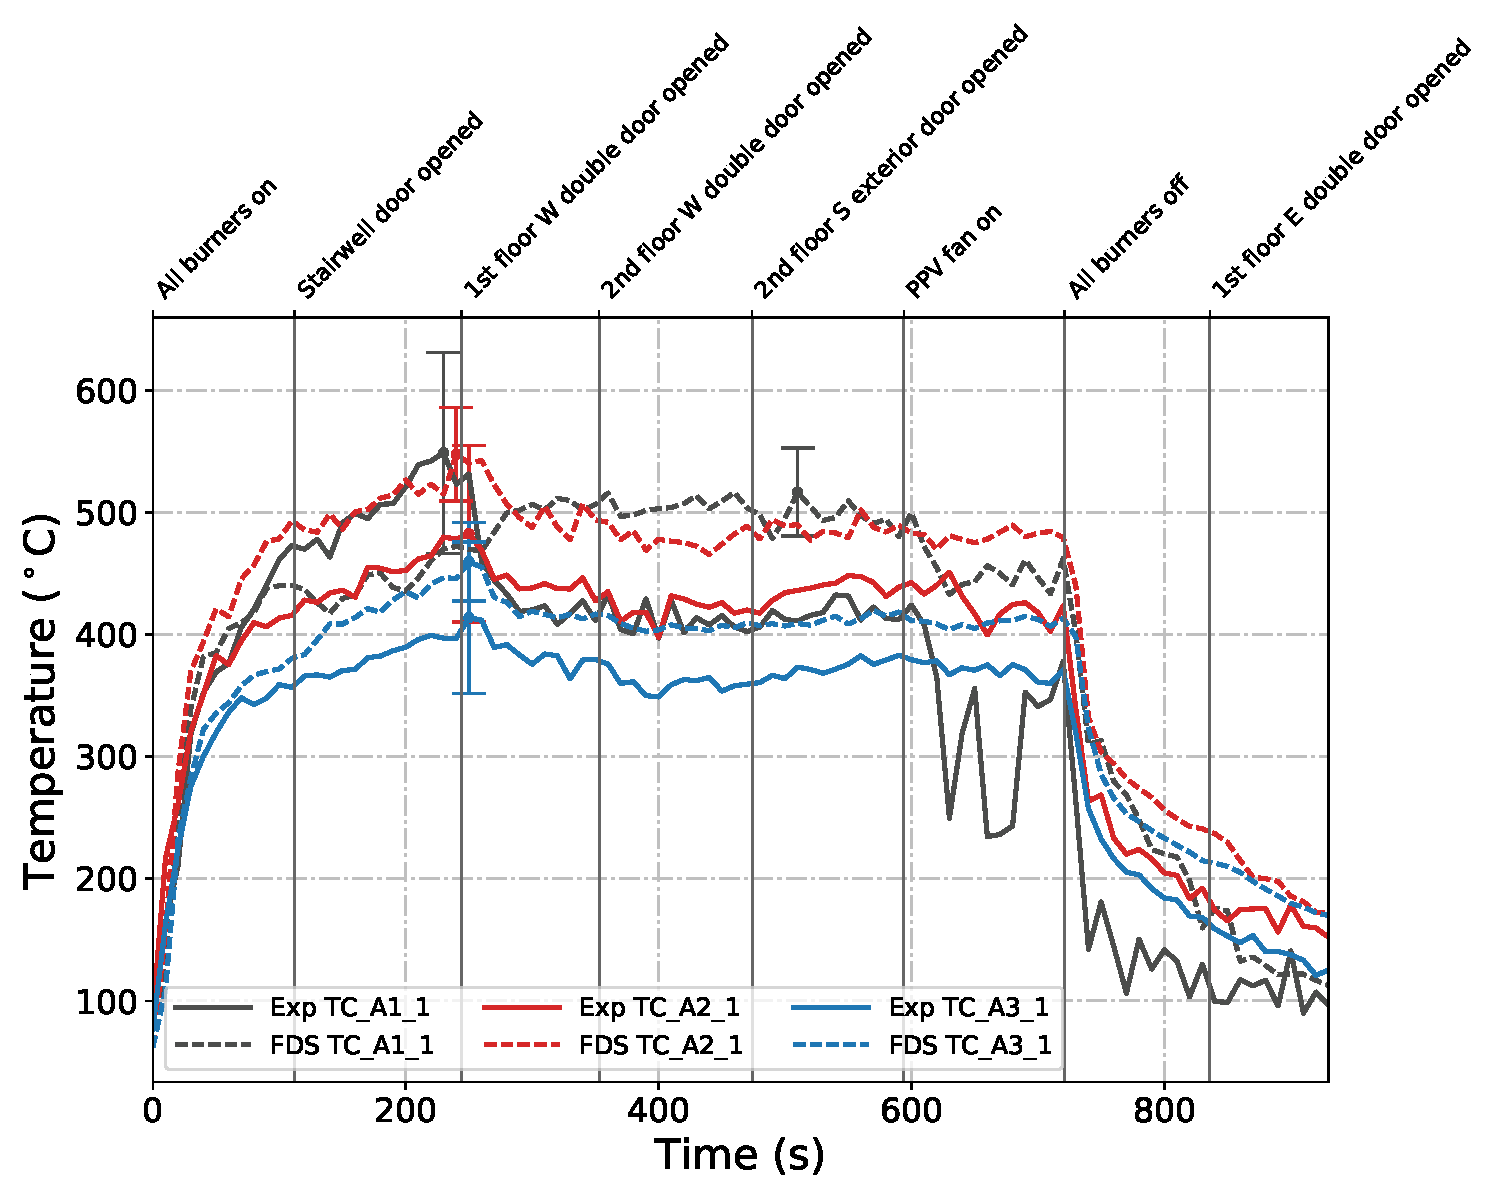
\includegraphics[width=0.87\columnwidth]{../../Plots/Grid_Sensitivity/Temperature/Test_25_cjet_1}
	\\~\\
	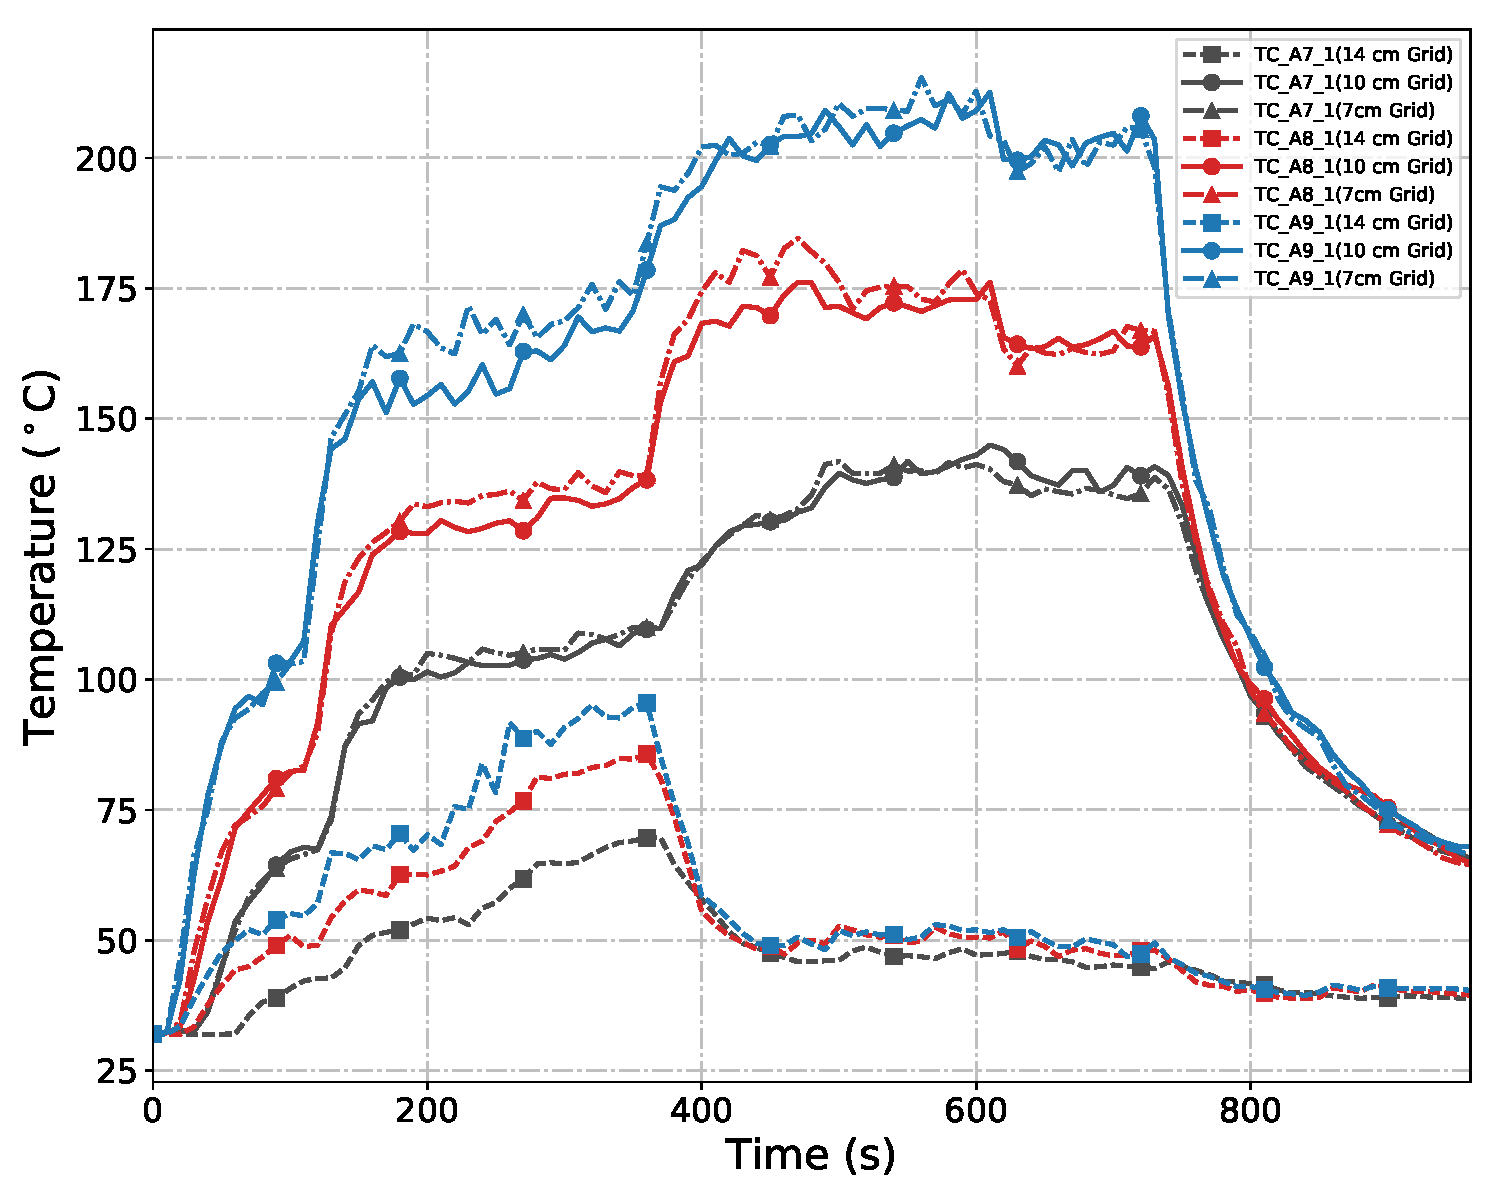
\includegraphics[width=0.87\columnwidth]{../../Plots/Grid_Sensitivity/Temperature/Test_25_cjet_2}
	\caption[Ceiling jet temperatures for West Structure simulations of various mesh sizes.]{Ceiling jet temperatures output by the FDS simulations with various mesh sizes for Test~25 in the West Structure.}
	\label{fig:west_cjet_sensitivity}
\end{figure}

\FloatBarrier

Looking at the plots presented above, significant changes in the model data exist when the grid size is reduced from 14~cm to 10~cm. Notice in Figure~\ref{fig:west_cjet_sensitivity}, the 14~cm grid was not refined enough to define the thermocouple locations at 0.03~m below the ceiling. Insignificant changes occur in the output data between the 10~cm grid size and the finer grid size of 5~cm for Test~4 and 7~cm for Test~25. These results suggest that a mesh size of 10~cm is appropriate for the FDS simulations of experiments in both the East and West Structures.

\section{FDS Model Output Compared to Experimental Data}
In the following subsections, the temperature, gas species concentration, gas velocity, and heat flux measurements predicted by the FDS simulations are compared to the corresponding sensor data measured during the propane burner experiments. Two different types of plots are presented in each section below. 

First, a figure is presented in each section to show a comparison of sensor data from a specific test (solid line with circle markers) and the corresponding data output by FDS (dashed line with triangle markers). These types of plots were generated for data collected at each of the various measurement locations described in Chapter~\ref{chap:exp_setup} for each experiment. Appendix~\ref{chap:exp_FDS_plots} contains the remaining plots that compare the experimental data to the FDS data over the duration of each experiment. 

The second type of plot that was generated for each discussed quantity is a log/log scatter plot designed to evaluate the model uncertainty in predicting the respective quantity. The plot is similiar to those found within the FDS Validation guide~\cite{FDS_Validation_Guide}. The procedure followed to generate the plots and statistical data is briefly outlined below. Full details of the analysis are described in detail in by McGrattan and Toman in Ref.~\cite{McGrattan:Metrologia}.

Taking $M_i$ and $E_i$ to represent the change in the value of a quantity from its ambient at a specific time based on the data output by the FDS simulation and measured by instrumentation during the experiment, respectively, the mean and standard deviation of the distribution can be estimated by first calculating
\begin{equation} 
	\overline{\ln(M/E)}=\frac{1}{n} \sum_{i=1}^n \ln\left( \frac{M_i}{E_i} \right)
\end{equation}
Note, the natural logarithm function is used so that the variance of the random variable can be expressed in terms of the relative uncertainty. The assumption that $\ln(M/E)$ is normally distributed has been tested for each data type of interest by the developers of FDS, and the results are shown in the FDS Validation Guide. The standard deviation of the logarithm of a normally distributed random variable is approximately equal to the standard deviation divided by its mean, the relative standard deviation. The least squares estimate of the standard deviation of the combined distribution is defined as:
\begin{equation}
\label{eq:least_sqrs}
	\widetilde{\sigma}_m^2 + \widetilde{\sigma}_E^2 \approx \frac{1}{n-1}\sum_{i=1}^n \left[ \ln(M_i/E_i) - \overline{\ln(M/E)} \right]^2
\end{equation}
Using the pair of measured and predicted values with the known $\widetilde{\sigma}_E$, the expression on the right can be evaluated. Eq.~\ref{eq:least_sqrs} imposes a constraint on the experimental uncertainty value, $\widetilde{\sigma}_E$, and in combination with a second constraint that $\widetilde{\sigma}_M$ cannot be less than $\widetilde{\sigma}_E$ because it's impossible to show that the model is more accurate than the measurements against which it's compared, the following is produced:
\begin{equation}
	\widetilde{\sigma}_E^2 \leq \frac{1}{2}\textrm{Var}(\ln(M/E))
\end{equation}
Using the mean of the distribution, an estimate of a bias factor, $\delta$, which expresses the tendency of the model to over or under-predict the measured quantity, can be found:
\begin{equation}
	\delta \approx \exp\left( \overline{\ln(M/E)}+\frac{\widetilde{\sigma}_M^2}{2}-\frac{\widetilde{\sigma}_E^2}{2} \right)
\end{equation}

The values of $\delta$, $\sigma_M$, and $\sigma_E$ are reported with each log/log plot in the following sections. For each plot, the solid red line and solid black line represent the expected values for $M$ and $E$, respectively, and the dashed lines represent $\pm \sigma$, or standard deviations, of the corresponding color. Each plotted gray point on the log/log scatter plots was plotted based on the average values across the same 30 second experimental period calculated using the model (predicted) data and the experimental (measured) data. The only 30 second time periods for which points were plotted are those during which natural ventilation was the only type of ventilation (i.e., periods for which there was no PPV fan) and at least one gas burner was ignited. Table~\ref{table:stats_compare} in the final section of this chapter summarizes the calculated statistical values for each data type and how they compare to the same statistics contained in the FDS Validation Guide.

\subsection{Temperature}

\subsubsection*{\textit{Hot Gas Layer}}
A quantity that is commonly estimated for compartment fire scenarios is the location of the interface between the hot, smoke-laden upper layer and cooler, lower layer. Some fire models, such as two-zone models, calculate this value directly, along with the average temperature of the upper (hot gas) layer and lower layer. Being that it's a CFD model, FDS computes a continuous profile of temperature and thus, does not directly calculate the interface location or the average temperature of each layer. However, numerous techniques exist to estimate the layer height and average temperatures from a continuous vertical profile of temperature. The temperatures measured by the thermocouples in the vertical arrays throughout the experimental structures were used to define a vertical profile of temperature, $T(z)$, in which $z$ is the height above the floor ($z=0$ at the floor and $z=H$ at the room's ceiling). Then, the vertical temperature profile was used to estimate the hot gas layer temperature by a method developed by Janssens and Tran~\cite{Janssens:JFS1992}. Taking $T_u$ as the upper layer temperature, $T_l$ as the lower layer temperature, and $z_{int}$ as the hot gas layer interface height, the method is outlined below, starting with the calculation of the quantities $I_1$ and $I_2$
\begin{equation*}
	I_1 = \int^H_0 T(z)dz = (H-z_{int})T_u+z_{int}T_l
\end{equation*}
\begin{equation*}
	I_2 = \int^H_0 \frac{1}{T(z)}dz = (H-z_{int})\frac{1}{T_u}+z_{int}\frac{1}{T_l}
\end{equation*}
$I_1$ and $I_2$ are then used to solve for $z_{int}$ as follows
\begin{equation}
	z_{int}=\frac{T_l(I_1I_2-H^2)}{I_1+I_2 T_l^2-2T_l H}
\end{equation}
$T_l$ is the temperature in the lowest mesh cell (or thermocouple) and $T_u$ is the average upper layer temperature defined by
\begin{equation}
	(H-z_{int})T_u=\int^H_{z_{int}} T(z)dz
\end{equation}

Figure~\ref{fig:HGL_data} shows the hot gas layer temperature derived from experimental data plotted with the same quantity derived from the FDS simulation data for Test~22, and Figure~\ref{fig:loglog_HGL} shows the log/log scatter plot of the hot gas layer temperatures obtained from the predicted data from the FDS simulations compared to the values obtained by the measured data for the six applicable gas burner experiments. 

\begin{figure}[!h]
	\centering
	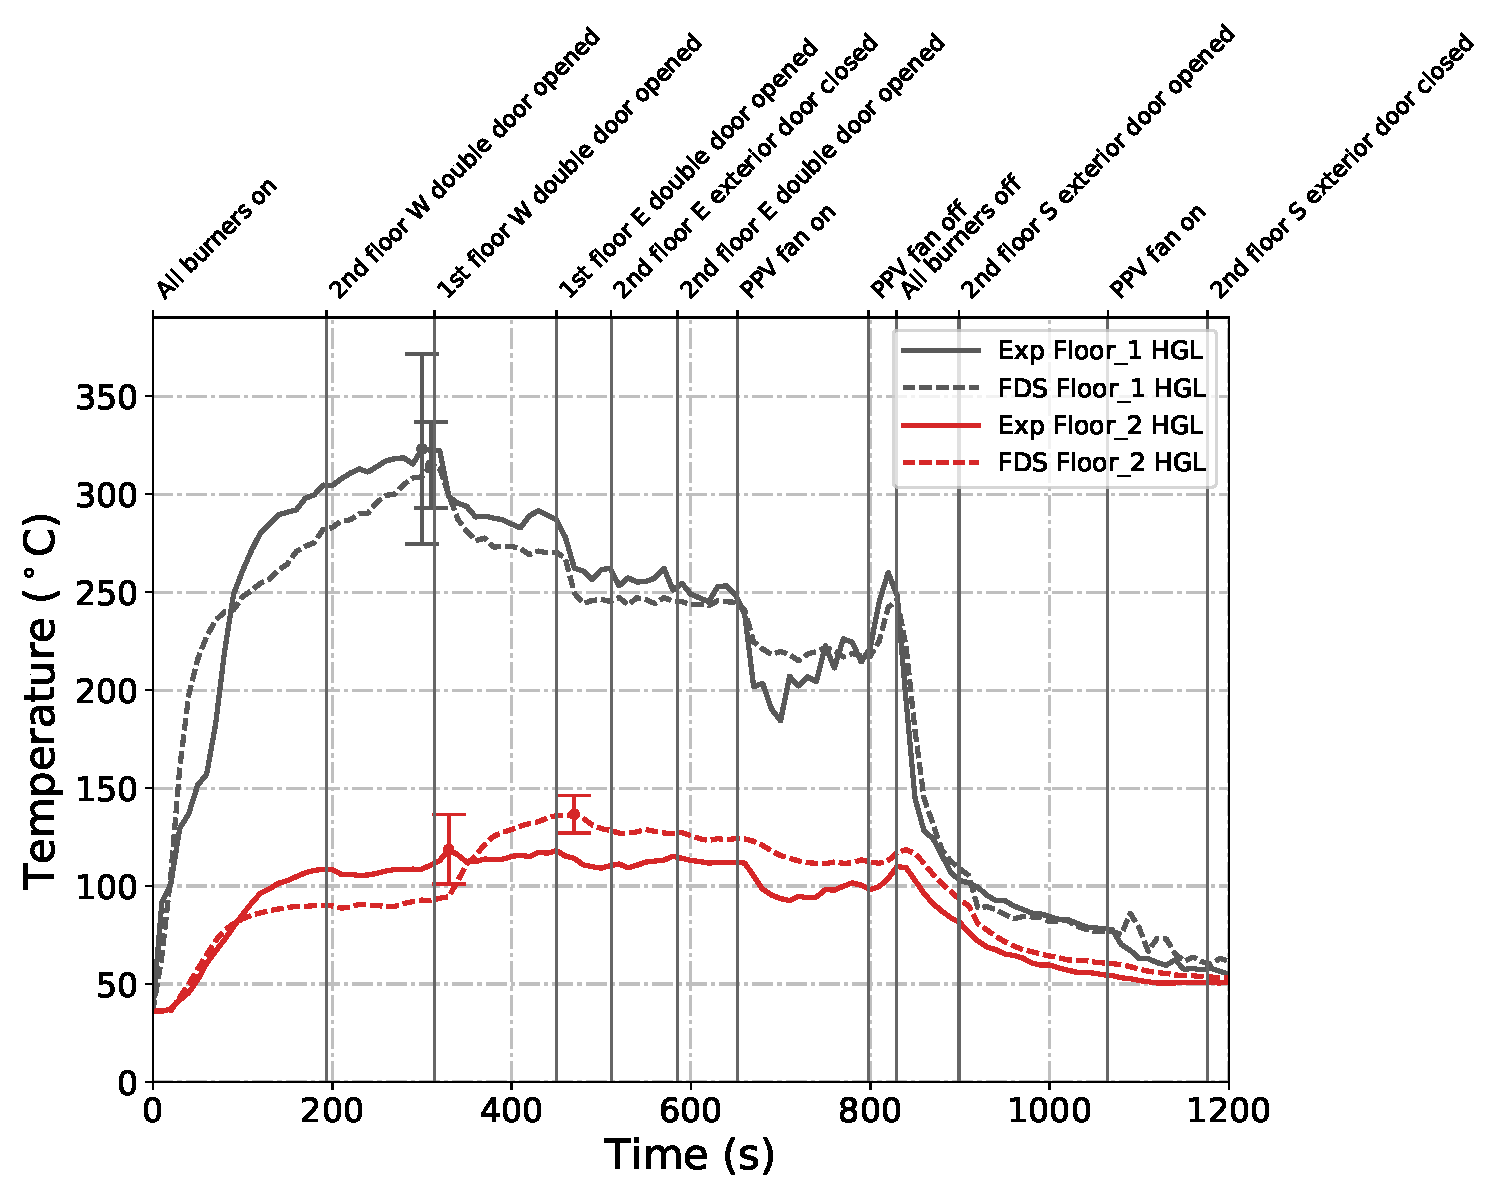
\includegraphics[width=\columnwidth]{../../Plots/Validation/Temperature/Test_22_HGL}
	\caption[Plots of measured and predicted hot gas layer temperatures during Test~22.]{Plots of measured and predicted hot gas layer temperatures on the first and second floors of the West Structure during Test~22.}
	\label{fig:HGL_data}
\end{figure}

\begin{figure}[!h]
	\centering
	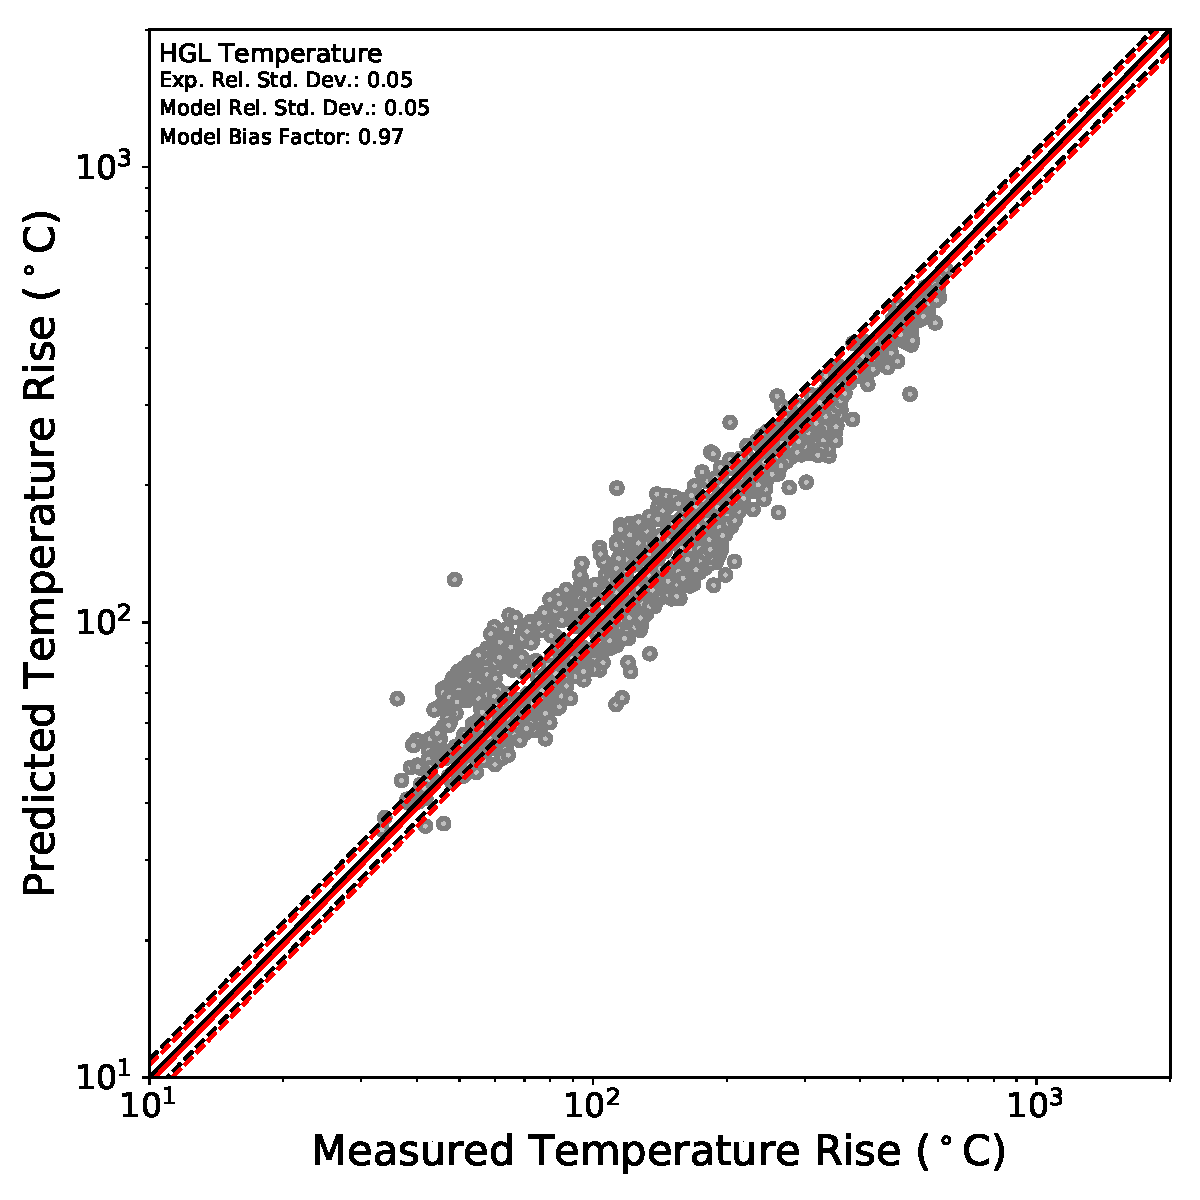
\includegraphics[width=\columnwidth]{../../Plots/Validation/Temperature/loglog_HGL}
	\caption{Summary of measured and predicted hot gas layer temperatures.}
	\label{fig:loglog_HGL}
\end{figure}

\FloatBarrier
\subsubsection*{\textit{Ceiling Jet}}
The temperature near the ceiling can be a used to evaluate a model's ability to predict the activation times of sprinklers, smoke detectors, and other fire protection devices at ceiling height. The ``ceiling jet'' temperature used throughout this report refers to the temperature measured by the top thermocouple (closest to the ceiling) of the various thermocouple arrays located throughout the experimental structures. Figure~\ref{fig:cjet_data} shows the ceiling jet temperatures measured during Test~4 plotted with the ceiling jet temperatures predicted by the FDS model for the same duration. Figure~\ref{fig:loglog_cjets} shows the log/log scatter plot of the ceiling jet temperatures predicted by the FDS simulations compared to the corresponding measured ceiling jet temperatures for the six applicable gas burner experiments.
\begin{figure}[!h]
	\centering
	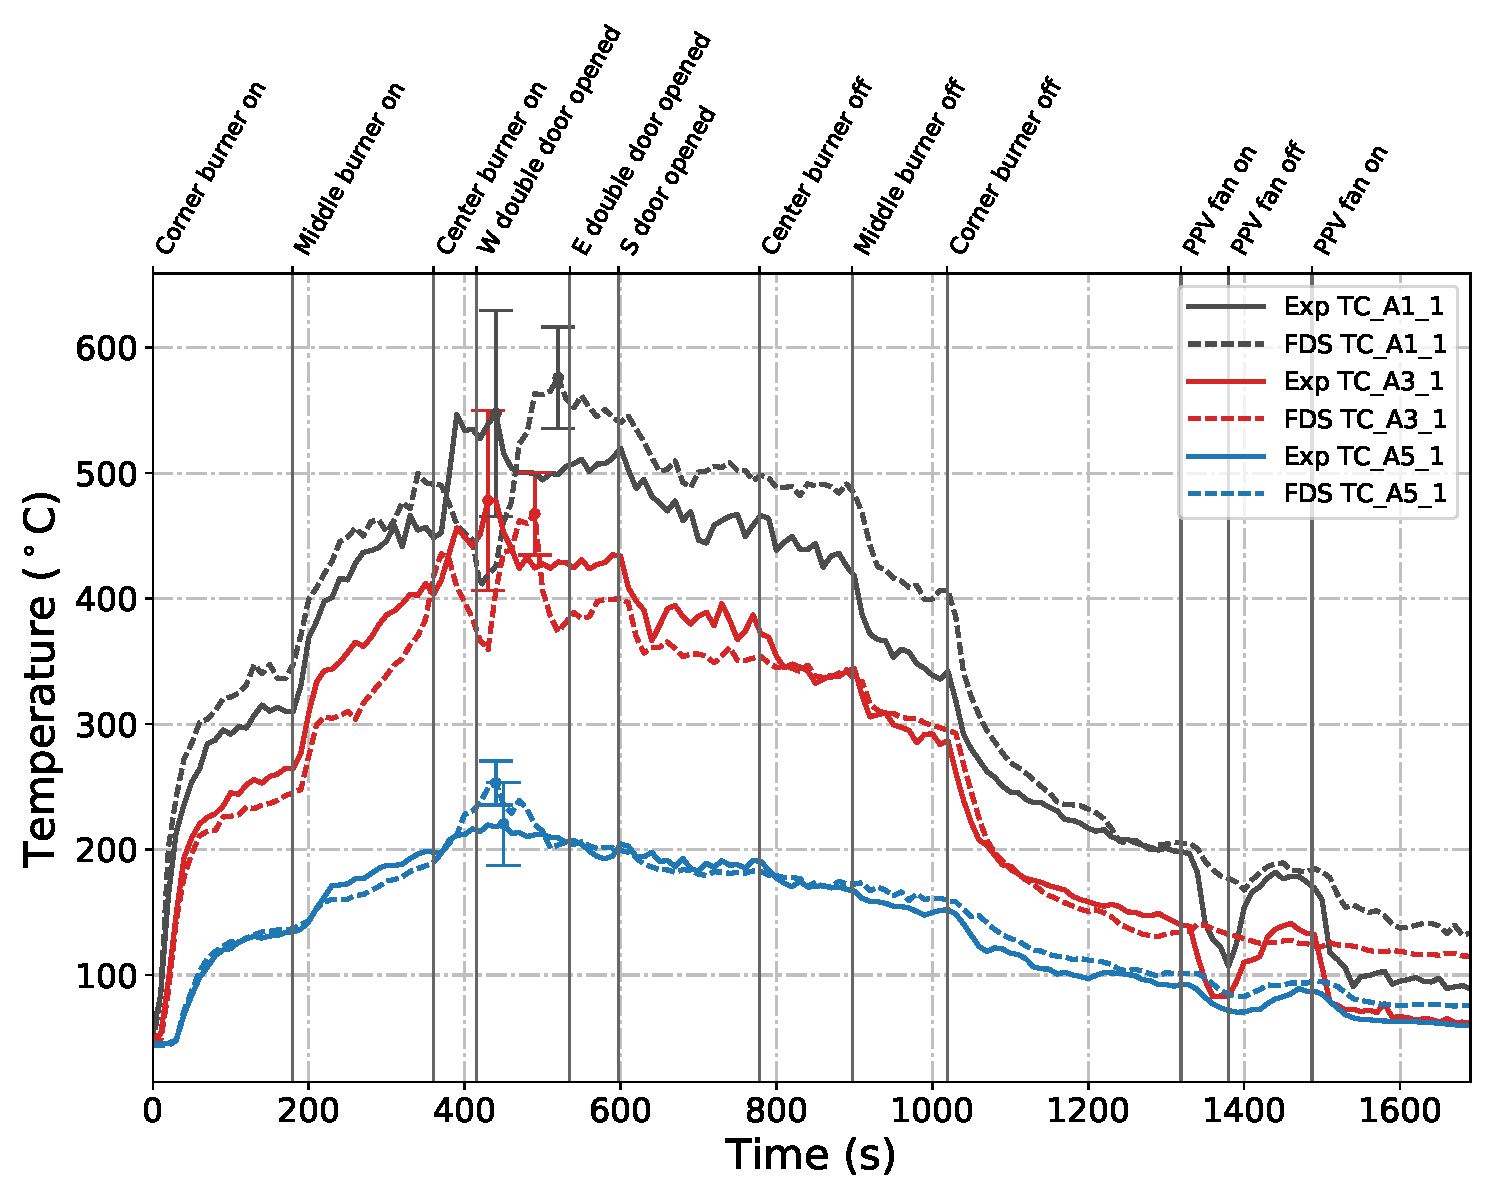
\includegraphics[width=\columnwidth]{../../Plots/Validation/Temperature/Test_4_cjet_1}
	\caption[Plots of measured and predicted ceiling jet temperatures during Test~4.]{Plots of measured and predicted ceiling jet temperatures during Test~4 obtained from thermocouple arrays A1, A3, and A5 located in the fire room, middle room, and north room, respectively.}
	\label{fig:cjet_data}
\end{figure}

\begin{figure}[!h]
	\centering
	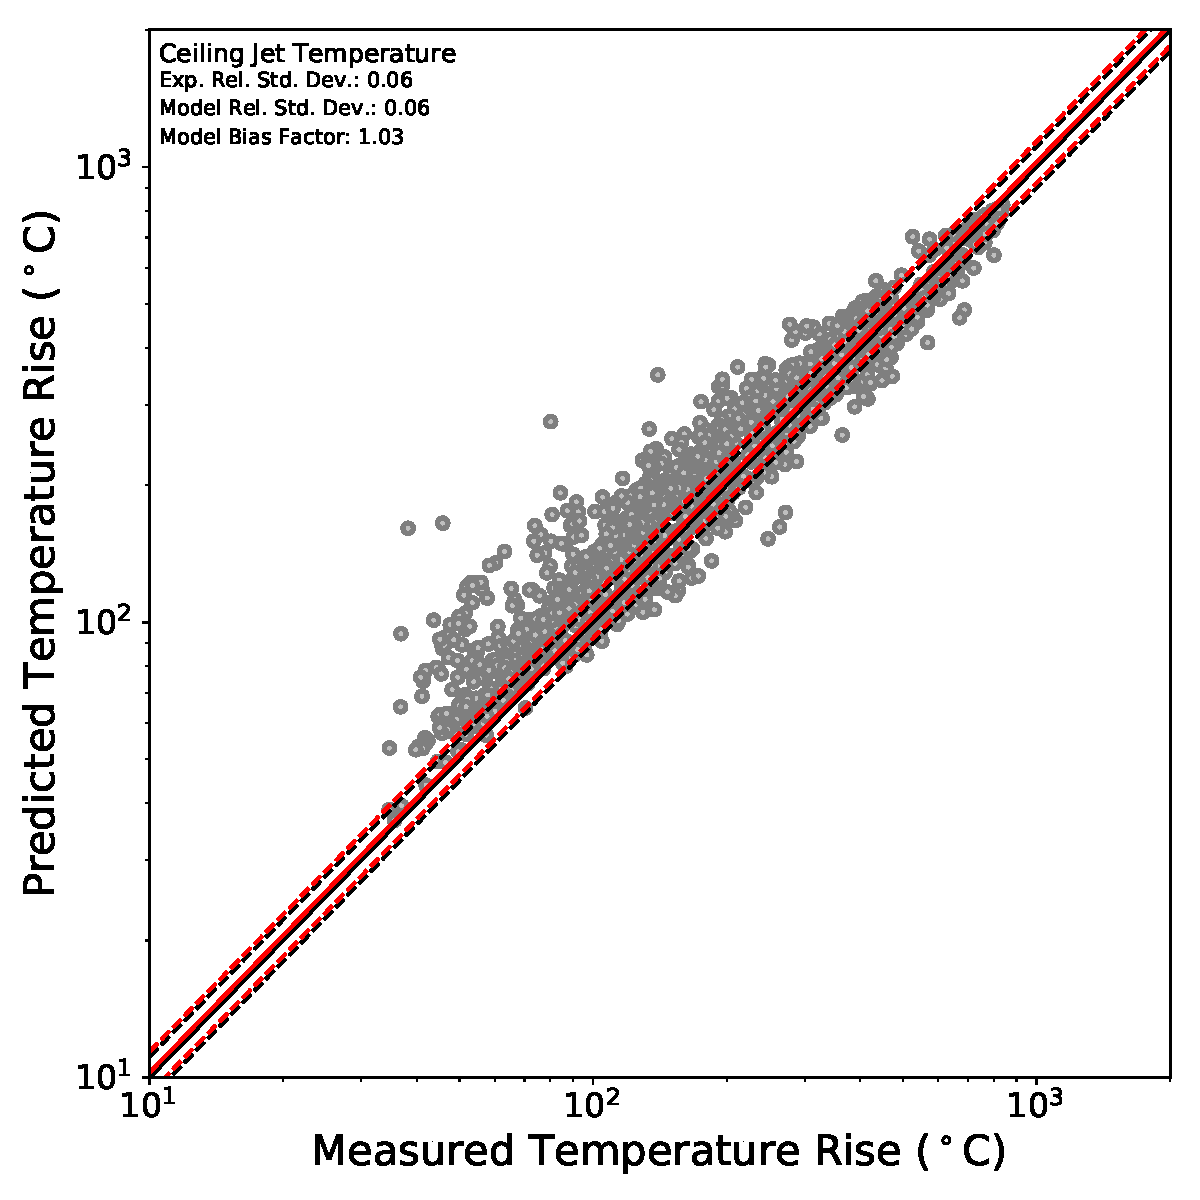
\includegraphics[width=\columnwidth]{../../Plots/Validation/Temperature/loglog_cjetTCs}
	\caption{Summary of measured and predicted ceiling jet temperatures.}
	\label{fig:loglog_cjets}
\end{figure}

\clearpage
\subsubsection*{\textit{Thermocouple Arrays}}
[PRESENT PLOTS SIMILAR TO HGL AND CEILING JET SECTIONS]
\begin{figure}[!h]
	\centering
	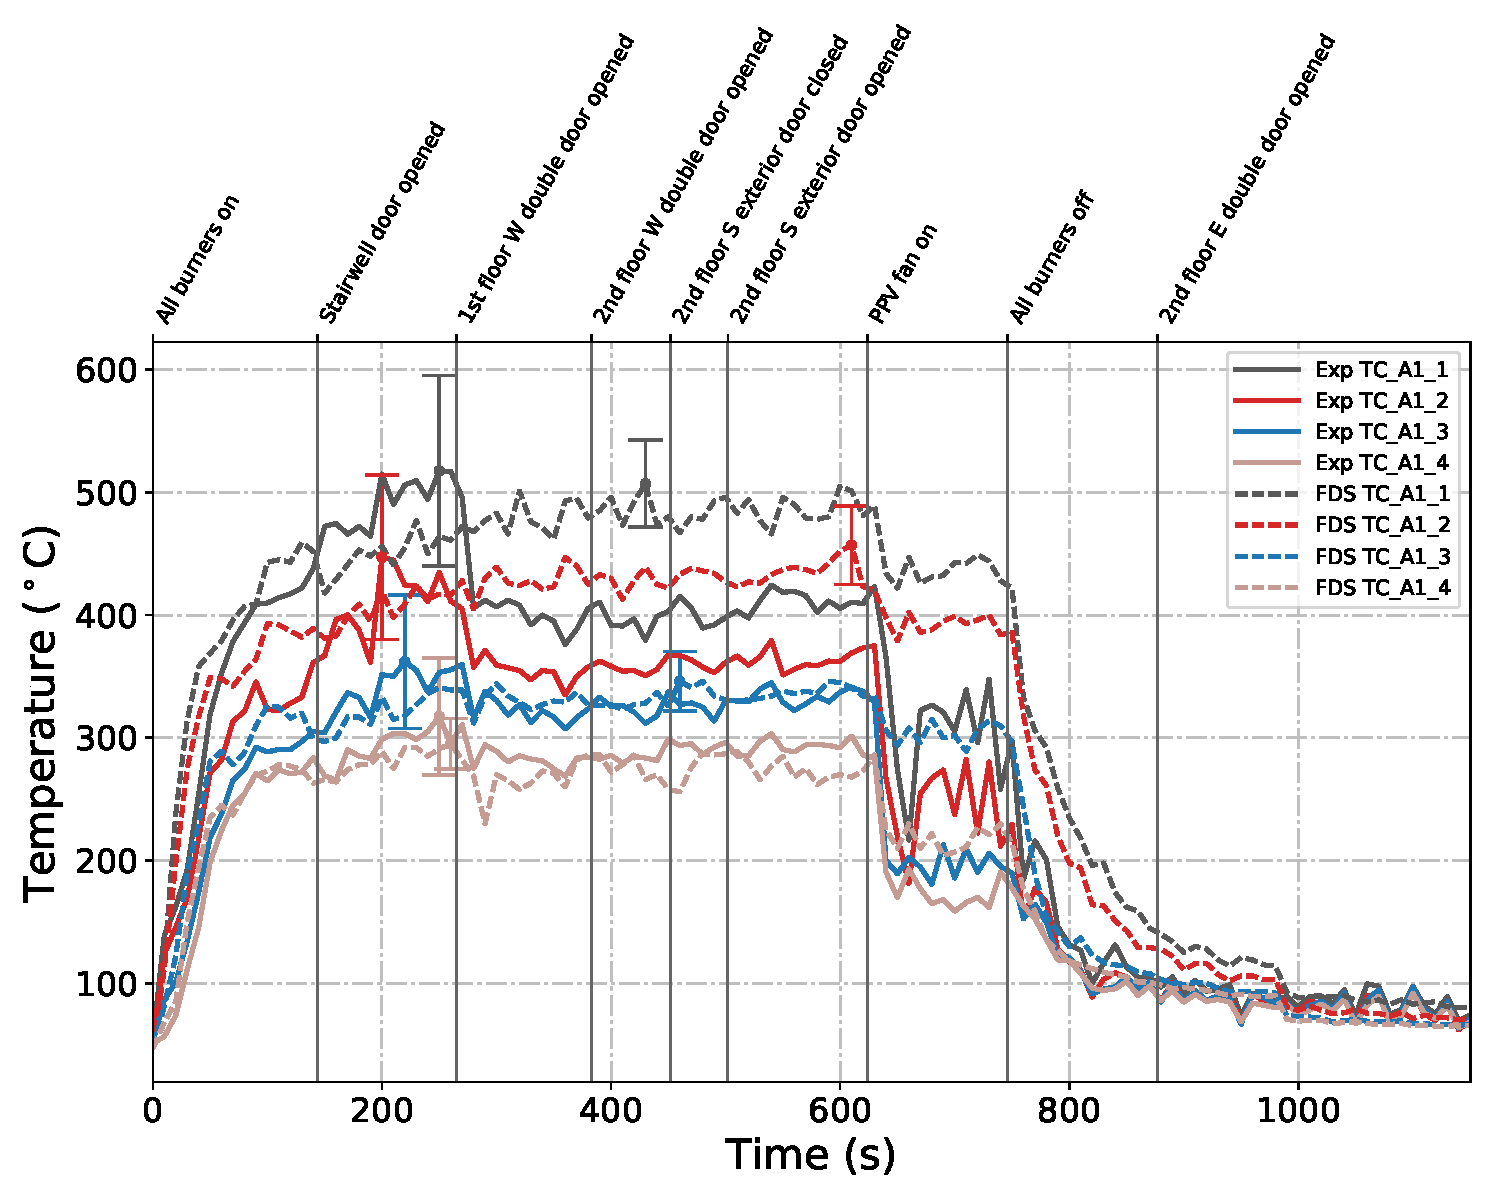
\includegraphics[width=\columnwidth]{../../Plots/Validation/Temperature/Test_24_TC_A1_upper}
	\caption[Plots of measured and predicted thermocouple array temperatures during Test~24.]{Plots of measured and predicted temperatures during Test~24 obtained from thermocouple array A1.}
	\label{fig:TCarray_data}
\end{figure}

\begin{figure}[!h]
	\centering
	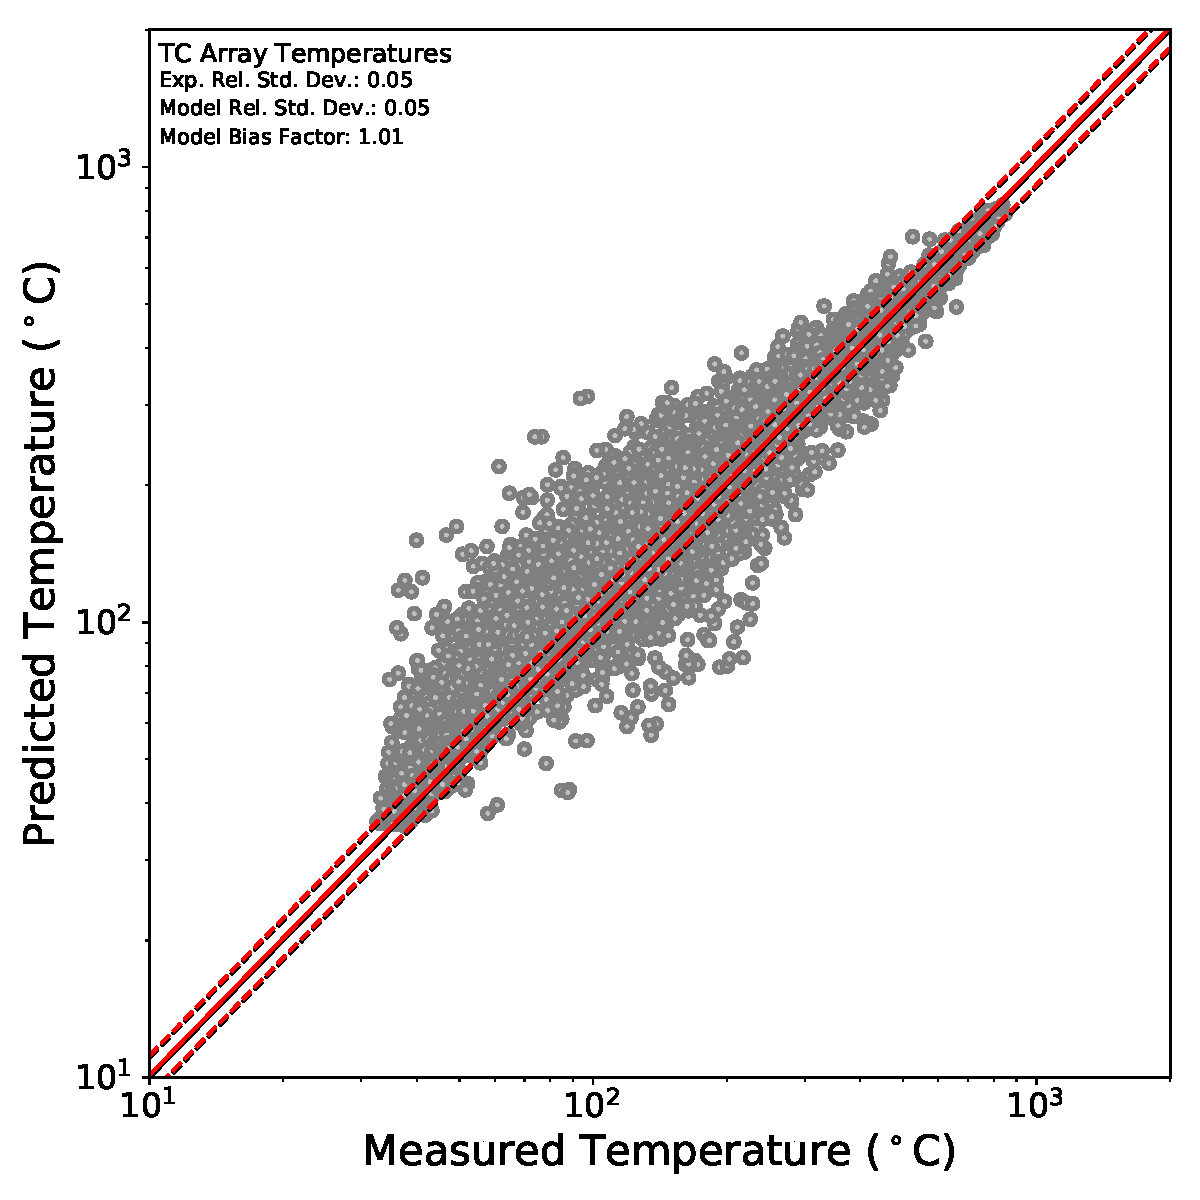
\includegraphics[width=\columnwidth]{../../Plots/Validation/Temperature/loglog_TC_arrays}
	\caption{Summary of measured and predicted temperatures obtained from thermocouple arrays.}
	\label{fig:loglog_TC_arrays}
\end{figure}

\clearpage
\subsection{Gas Species Concentration}

\subsubsection*{\textit{$O_2$} Concentration}
[PRESENT PLOTS SIMILAR TO HGL AND CEILING JET SECTIONS]
\begin{figure}[!h]
	\centering
	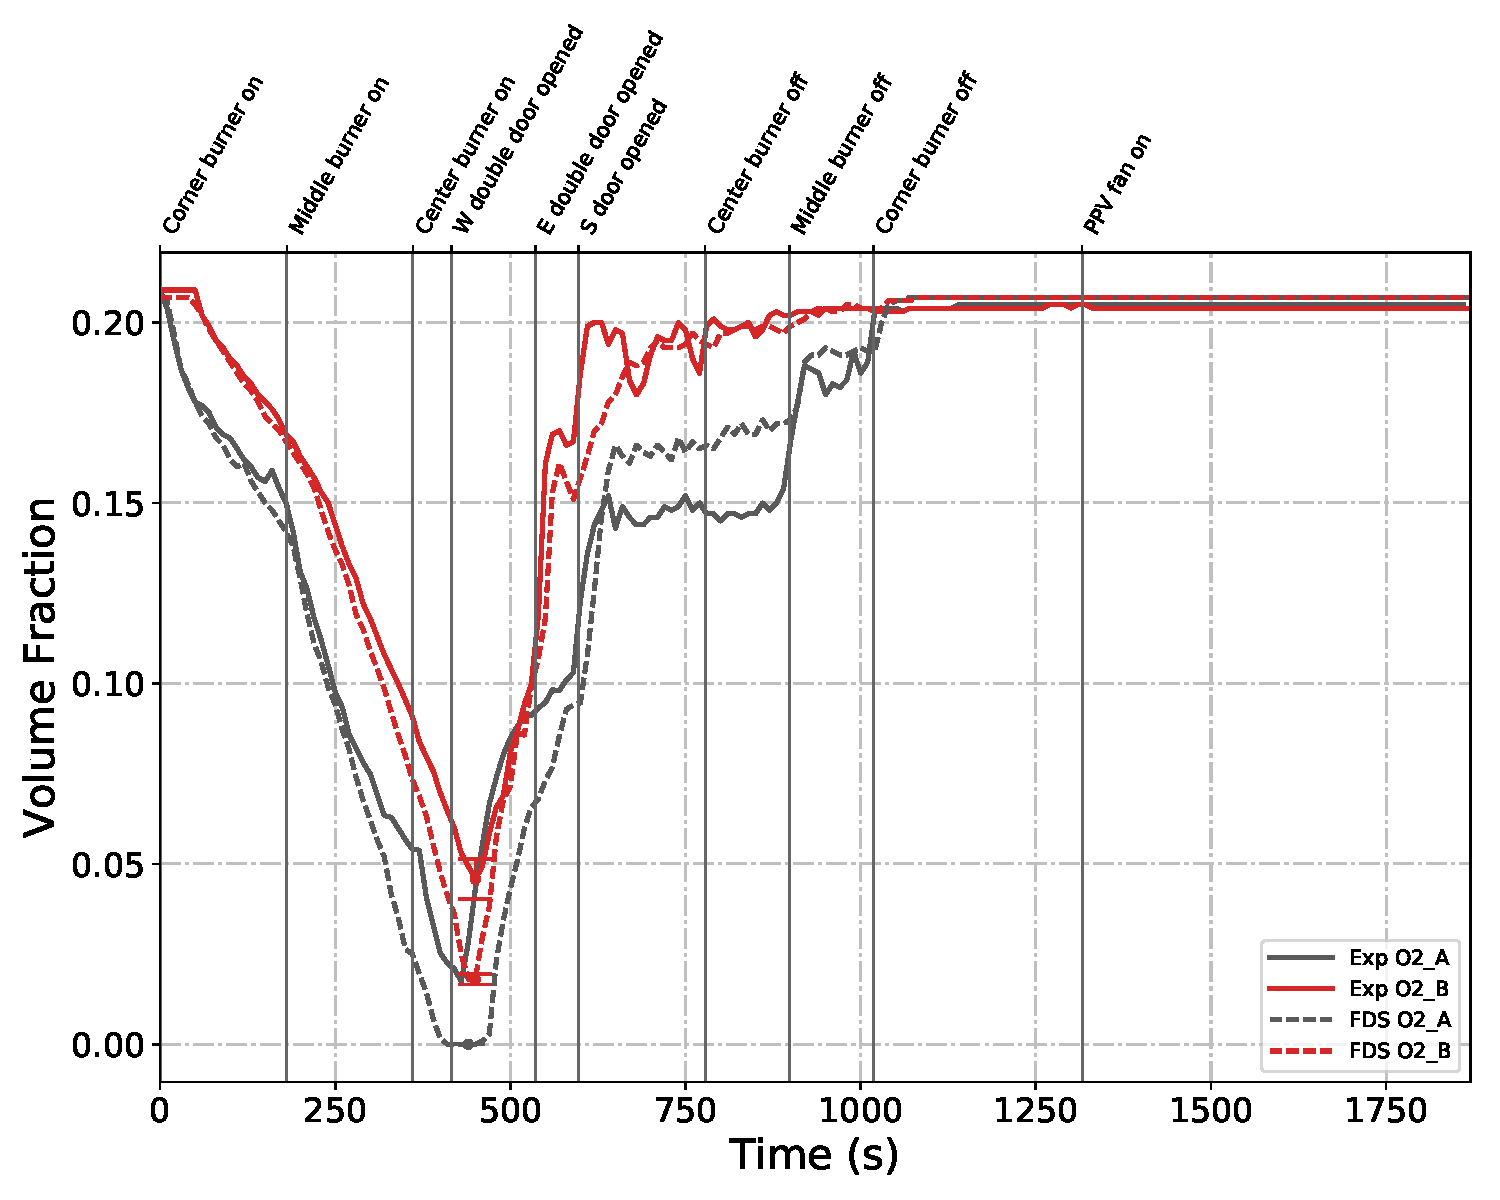
\includegraphics[width=\columnwidth]{../../Plots/Validation/Gas_Concentration/Test_3_O2}
	\caption[Plots of measured and predicted $O_2$ concentration during Test~3.]{Plots of measured and predicted $O_2$ concentration in the fire room (black plots) and north room (red plots) during Test~3.}
	\label{fig:Test3_O2}
\end{figure}

\begin{figure}[!h]
	\centering
	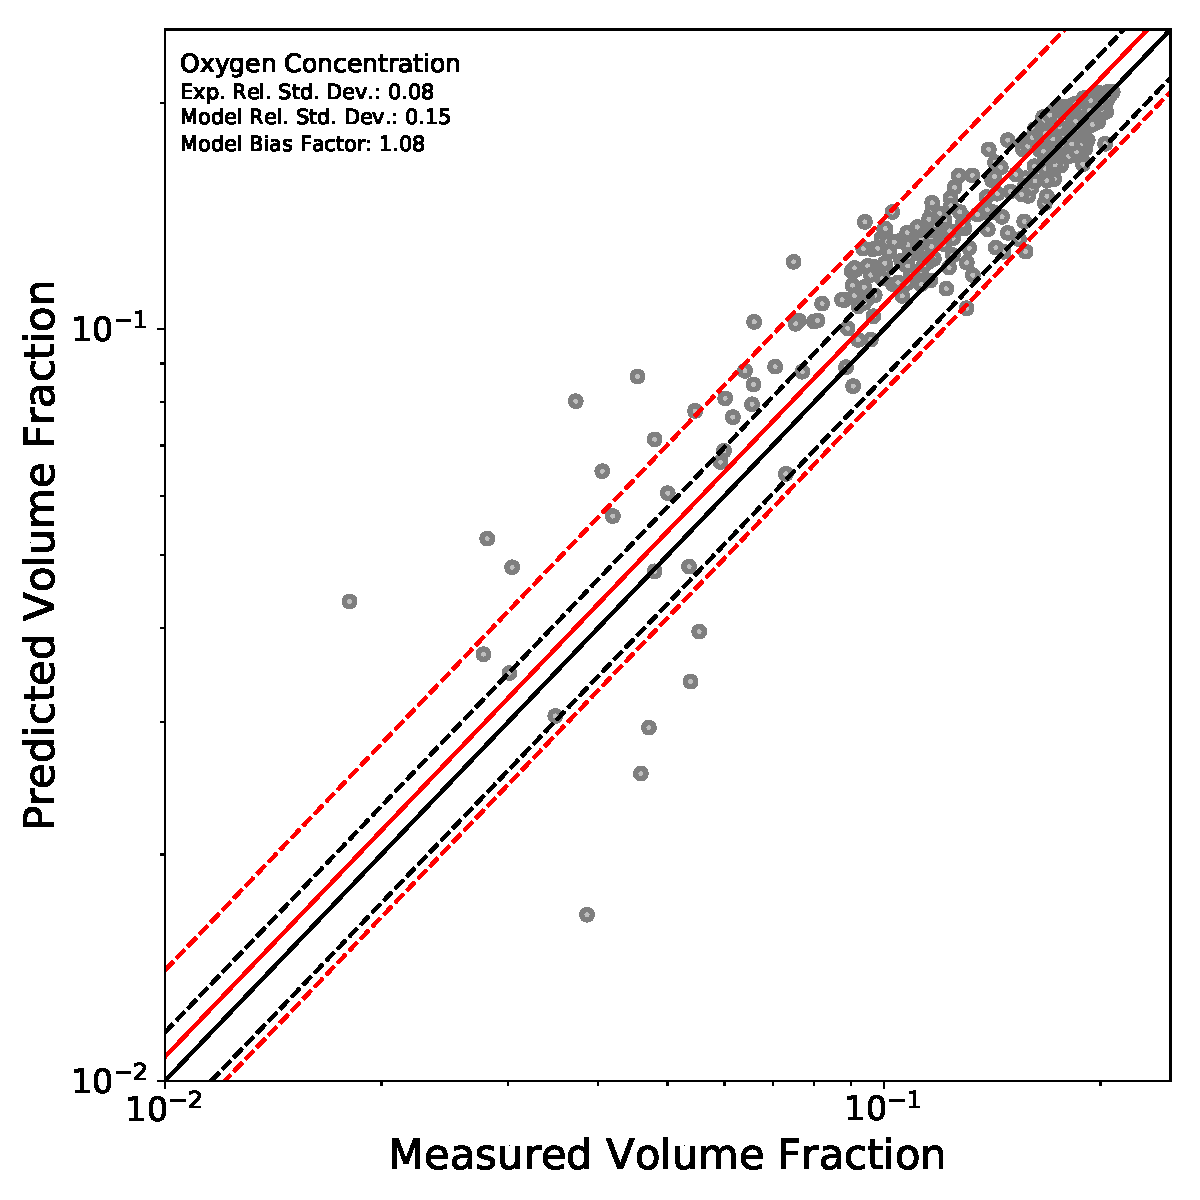
\includegraphics[width=\columnwidth]{../../Plots/Validation/Gas_Concentration/loglog_O2}
	\caption{Summary of measured and predicted $O_2$ concentrations.}
	\label{fig:loglog_O2}
\end{figure}

\FloatBarrier
\subsubsection*{\textit{$CO_2$} Concentration}
Note about maximum reading of 0.10 due to instrumentation. [PRESENT PLOTS SIMILAR TO HGL AND CEILING JET SECTIONS]
\begin{figure}[!h]
	\centering
	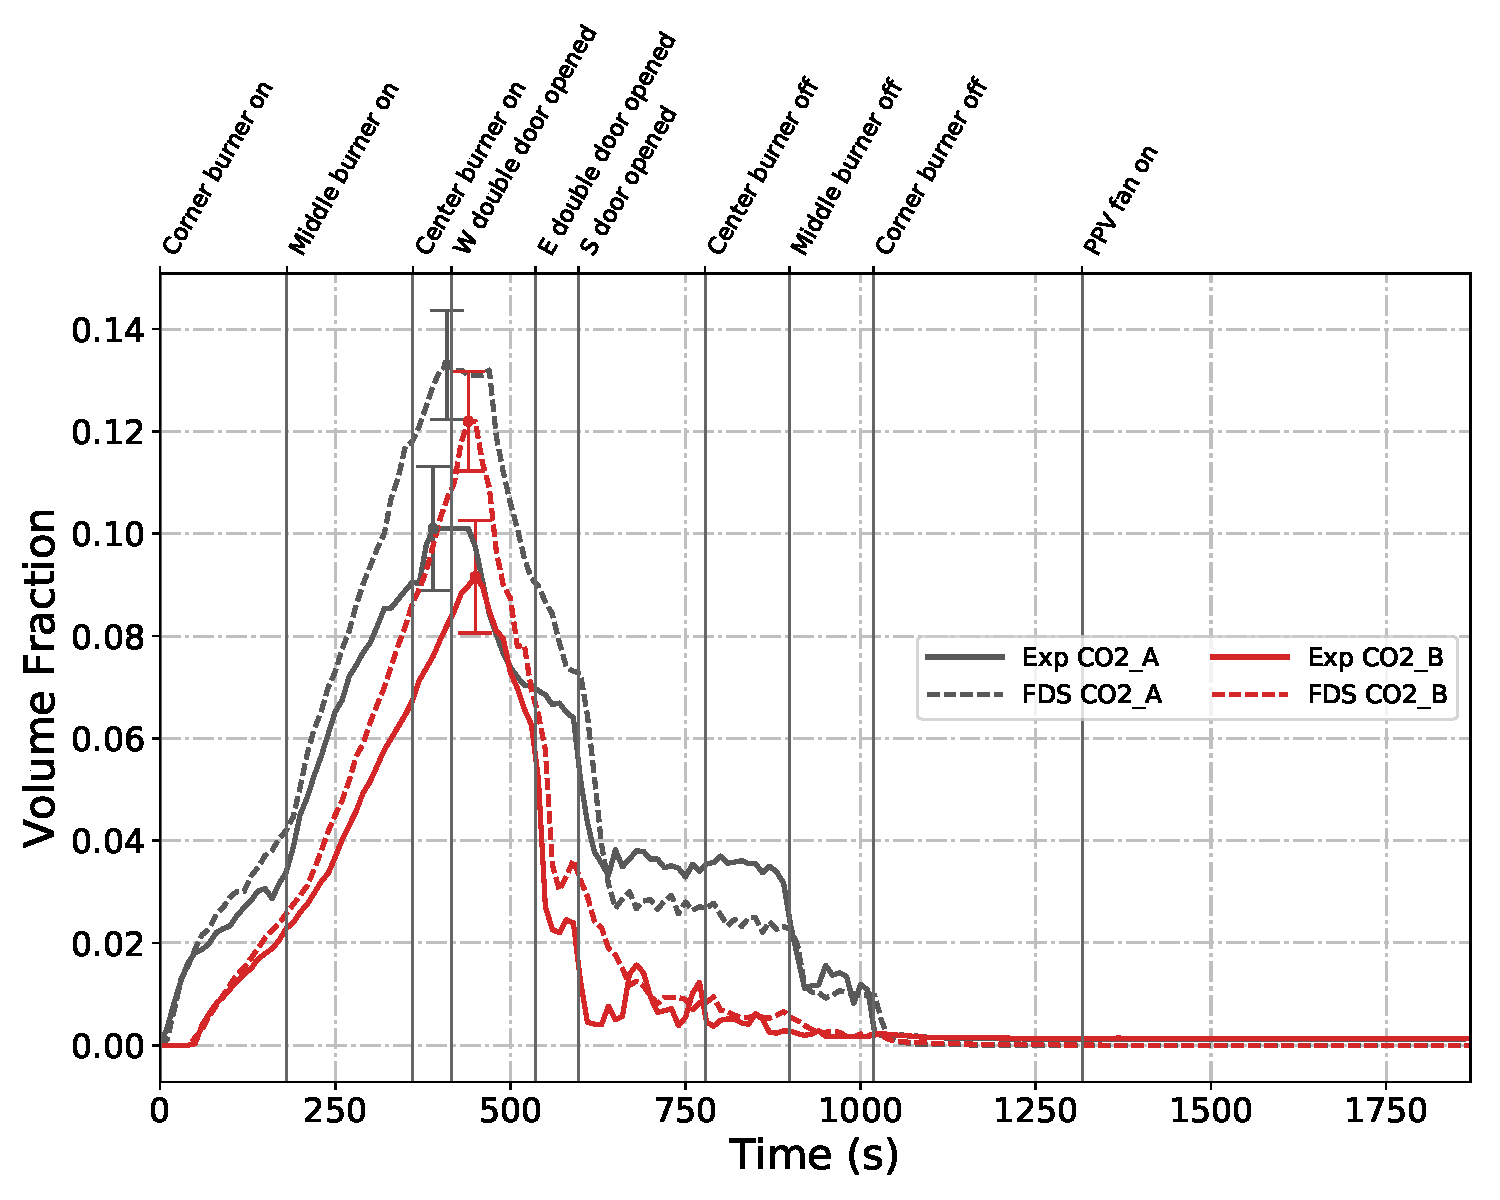
\includegraphics[width=\columnwidth]{../../Plots/Validation/Gas_Concentration/Test_3_CO2}
	\caption[Plots of measured and predicted $CO_2$ concentration during Test~3.]{Plots of measured and predicted $CO_2$ concentration in the fire room (black plots) and north room (red plots) during Test~3.}
	\label{fig:Test3_CO2}
\end{figure}

\begin{figure}[!h]
	\centering
	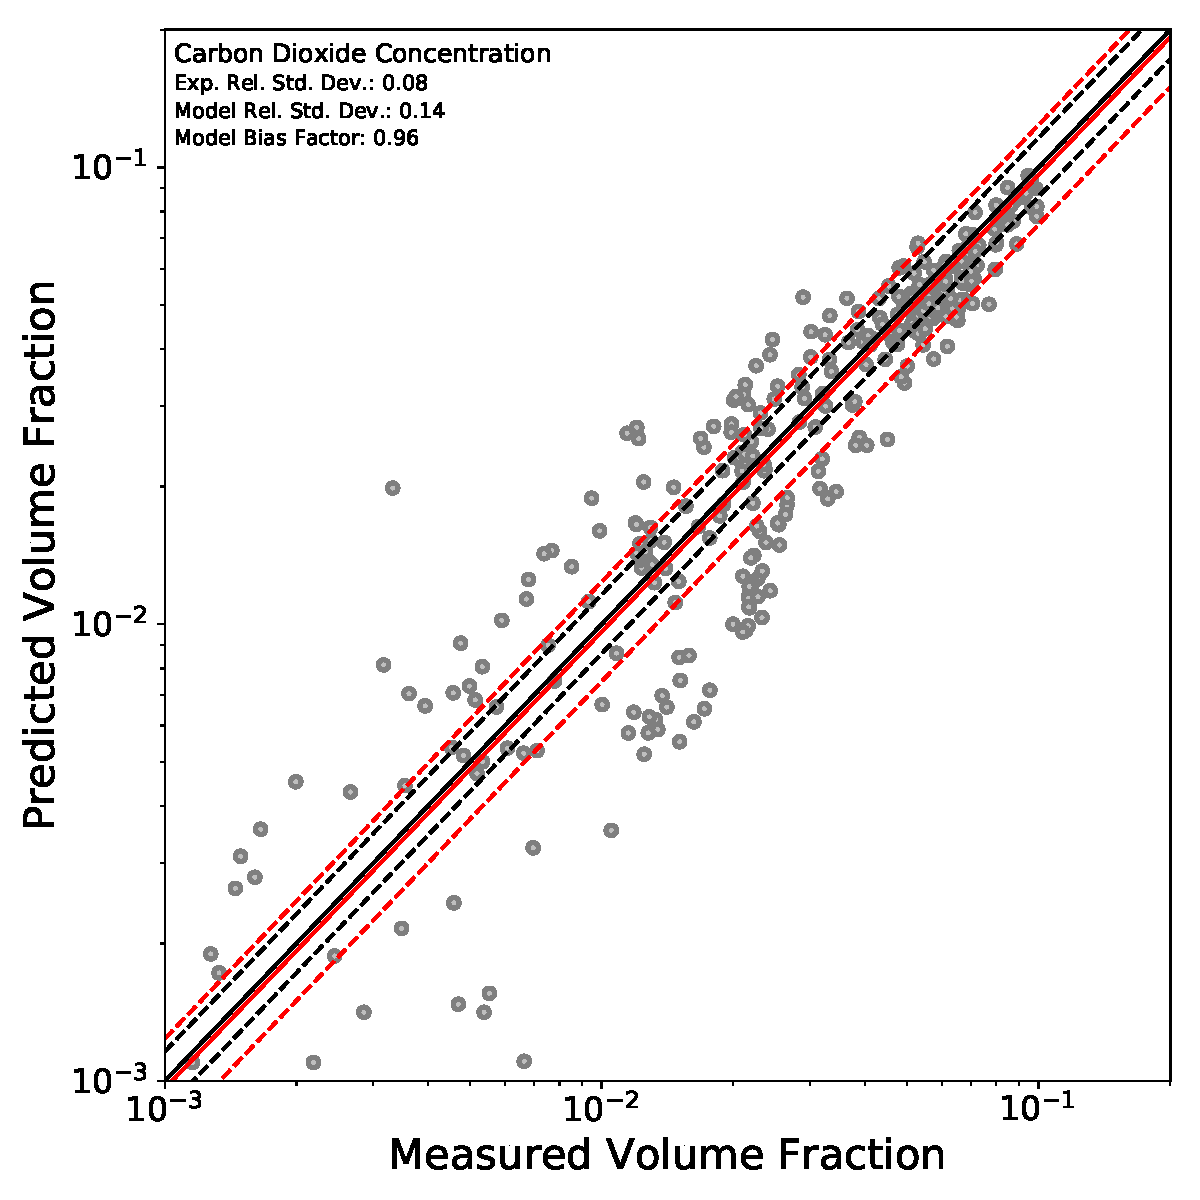
\includegraphics[width=\columnwidth]{../../Plots/Validation/Gas_Concentration/loglog_CO2}
	\caption{Summary of measured and predicted $CO_2$ concentrations.}
	\label{fig:loglog_CO2}
\end{figure}

\clearpage
\subsection{Gas Velocity}
Because the gas burner experiments were conducted outdoors, they were subject to environmental conditions, such as wind. To minimize the effect such environmental conditions could have on the analysis of the results, the only gas velocity measurements that are considered in this section are those that were indoors, or well-protected from the exterior. The one gas velocity measurement location in the East Structure that was well-protected from the effects of environmental conditions is the location at the roof vent, the set of three BDPs at the location A10. Tests~5 and 6 were the only East Structure tests that incorporated the roof vent as a ventilation opening. Similarly, there was only one set of BDPs in the West Structure that was well protected from the exterior environment: the set of eight BDPs at the top of the stairs at measurement location A10. All four tests conducted in the West Structure used the stairwell door as a ventilation opening. For Tests~22 and 23, the door was in the open position the entire duration of the experiments, and for Tests~24 and 25, the door was opened at a point during the test. Only the measured and predicted data corresponding to when the door was in the open position is considered in the analysis below. 

\begin{figure}[!h]
	\centering
	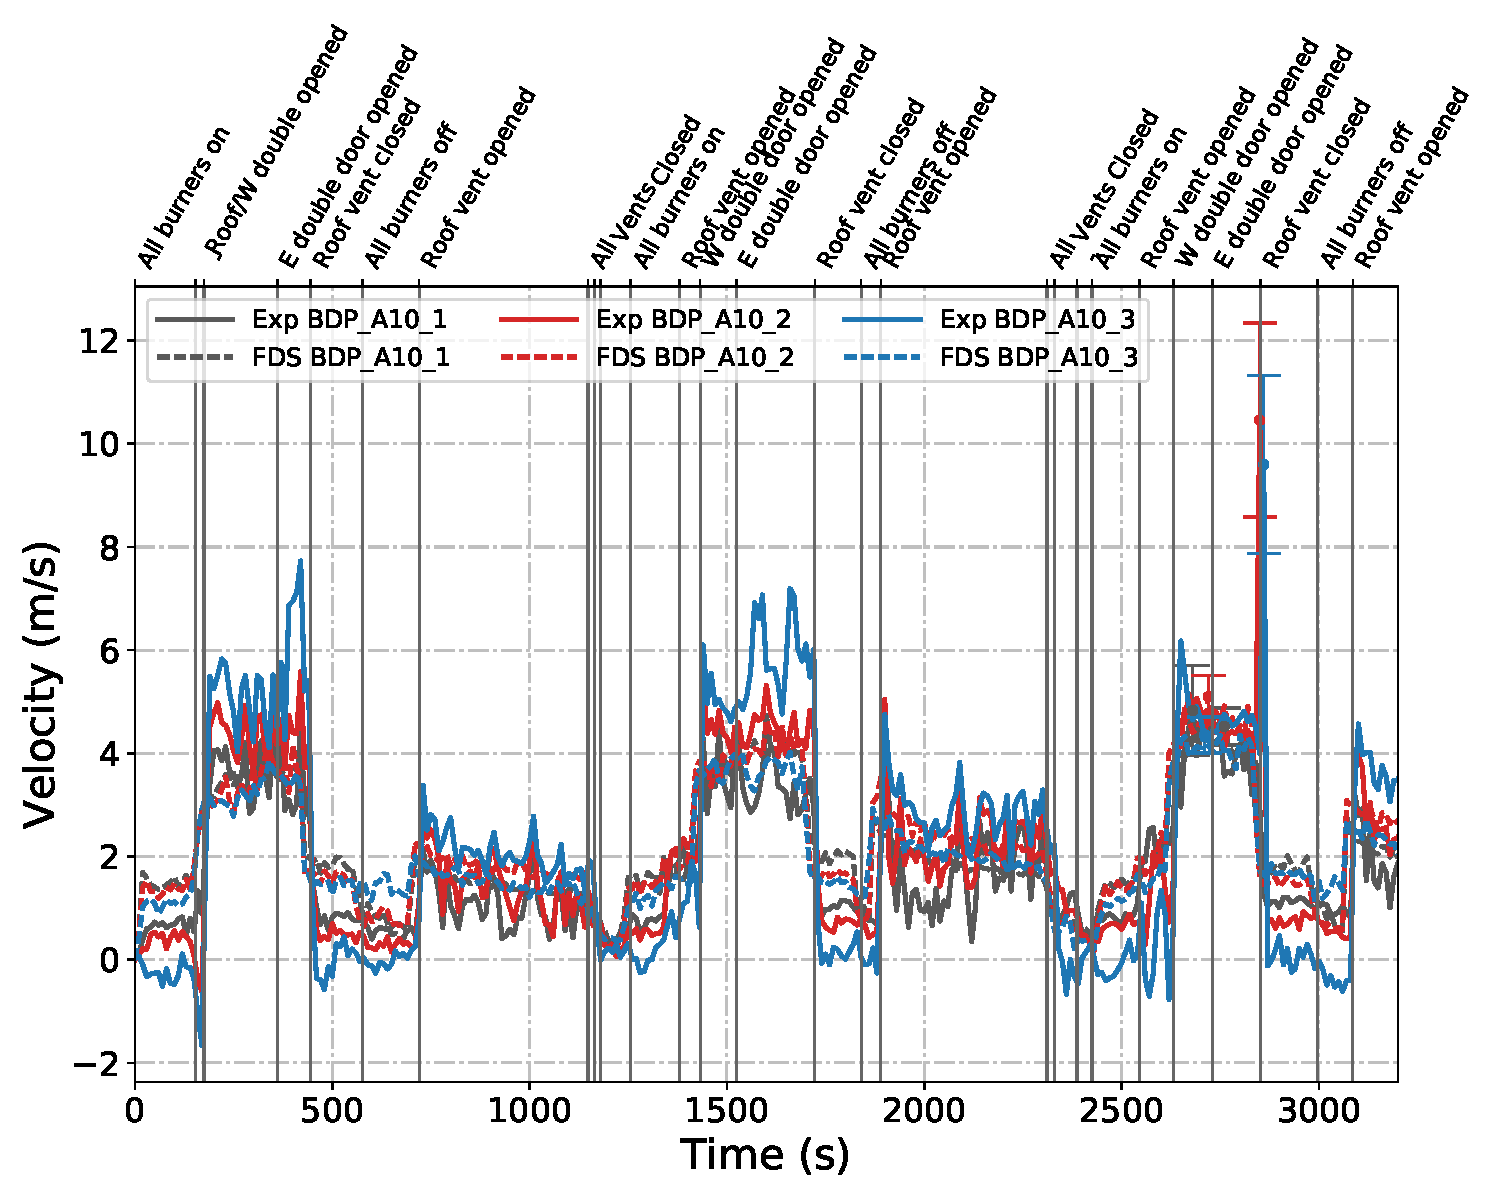
\includegraphics[width=\columnwidth]{../../Plots/Validation/Velocity/Test_5_BDP_A10}
	\caption[Plots of measured and predicted gas velocity through the roof vent during Test~5.]{Plots of measured and predicted gas velocity through the roof vent during Test~5.}
	\label{fig:Test5_BDPs}
\end{figure}

\begin{figure}[!h]
	\centering
	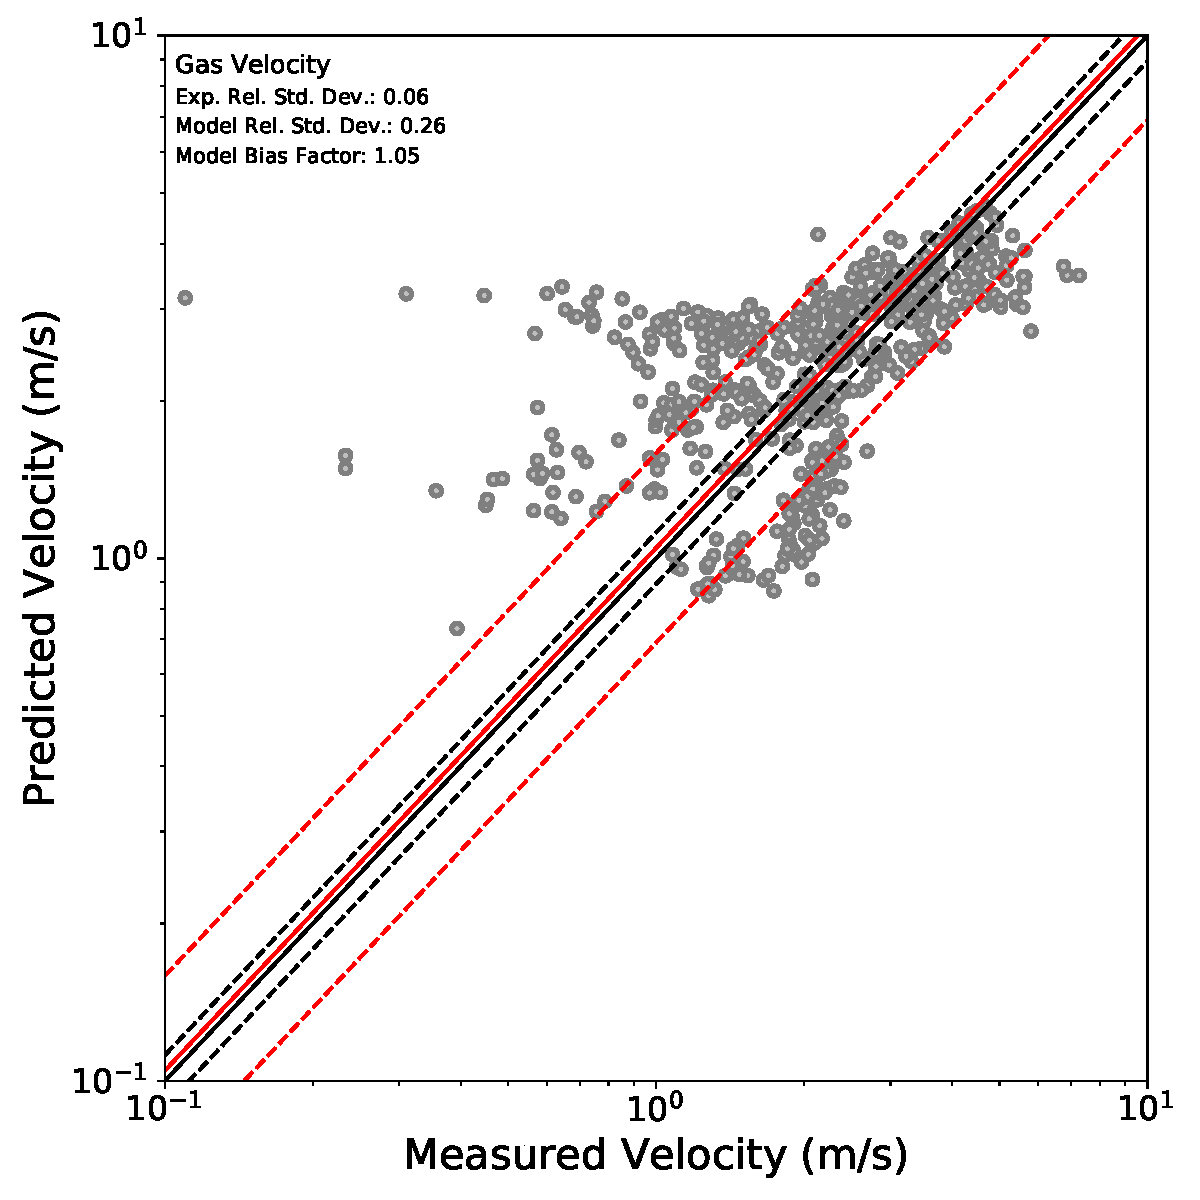
\includegraphics[width=\columnwidth]{../../Plots/Validation/Velocity/loglog_BDPs}
	\caption{Summary of measured and predicted gas velocity measurements.}
	\label{fig:loglog_BDPs}
\end{figure}

\clearpage
\subsection{Total Heat Flux}
[PRESENT PLOTS SIMILAR TO HGL AND CEILING JET SECTIONS]
\begin{figure}[!h]
	\centering
	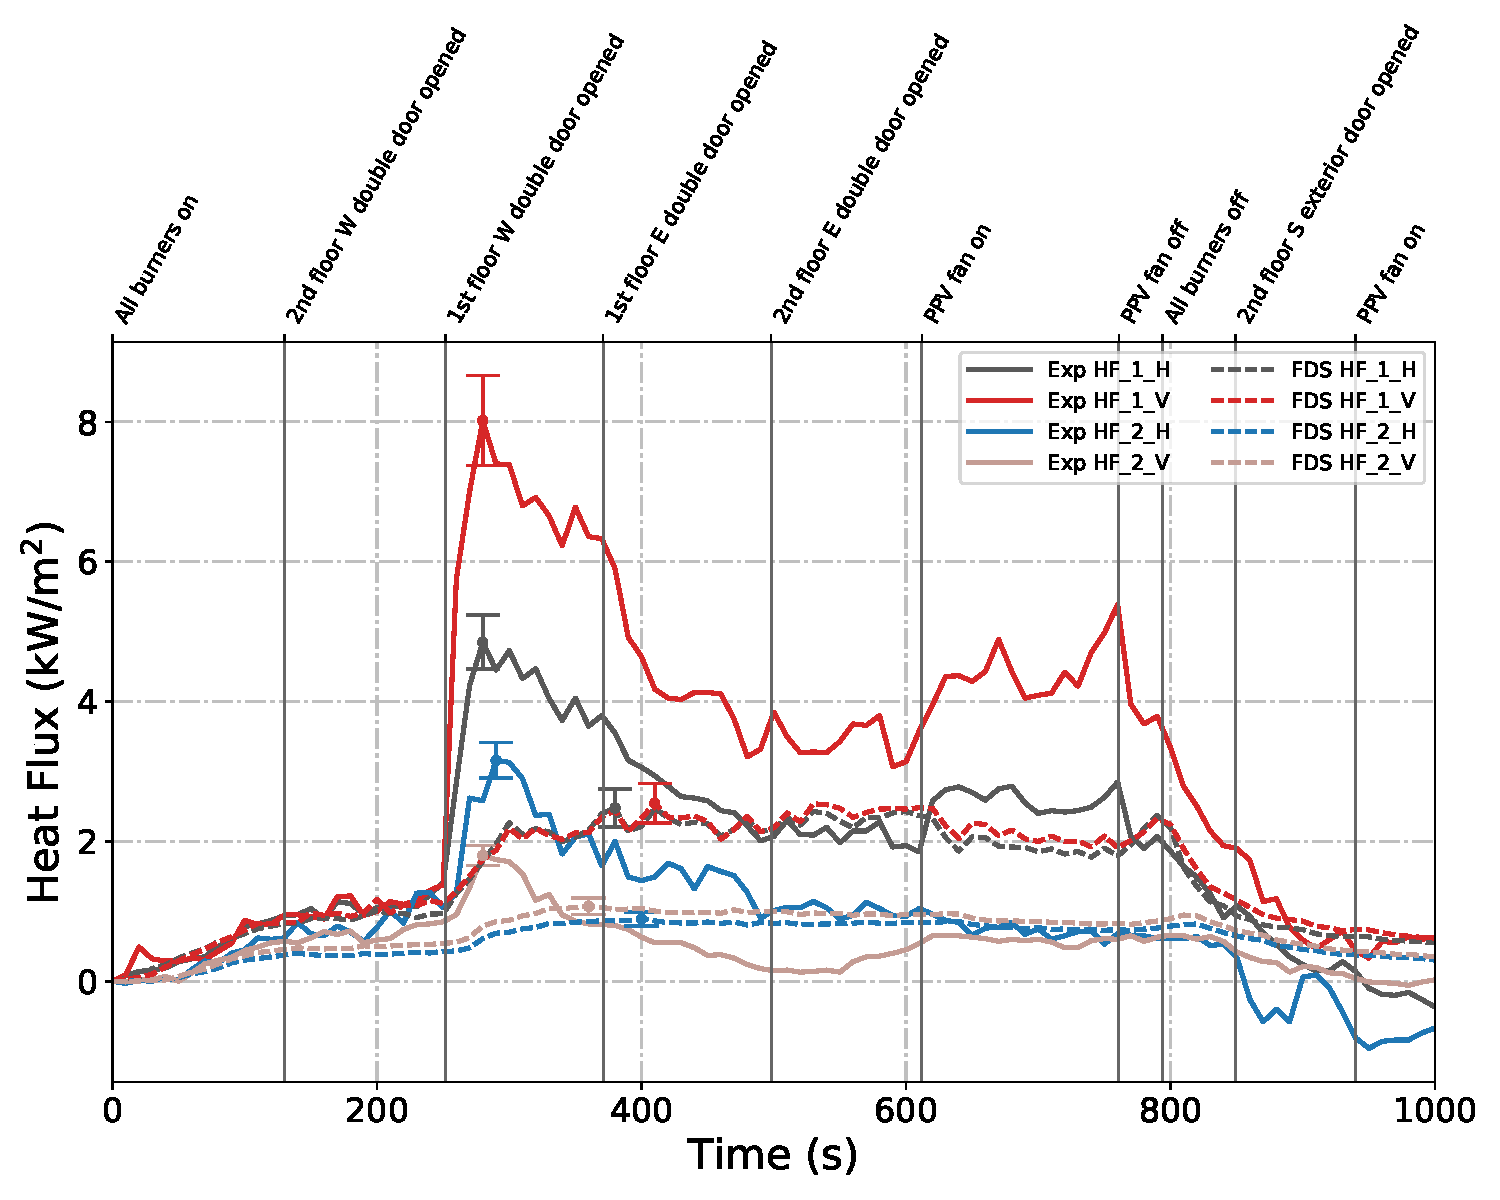
\includegraphics[width=\columnwidth]{../../Plots/Validation/Heat_Flux/Test_23_HFs}
	\caption[Plots of measured and predicted heat flux during Test~23.]{Plots of measured and predicted heat flux measured by total heat flux gauges at the top of the stairs facing the stair doorway (`H') and facing the ceiling (`V').}
	\label{fig:Test23_HF1}
\end{figure}

\begin{figure}[!h]
	\centering
	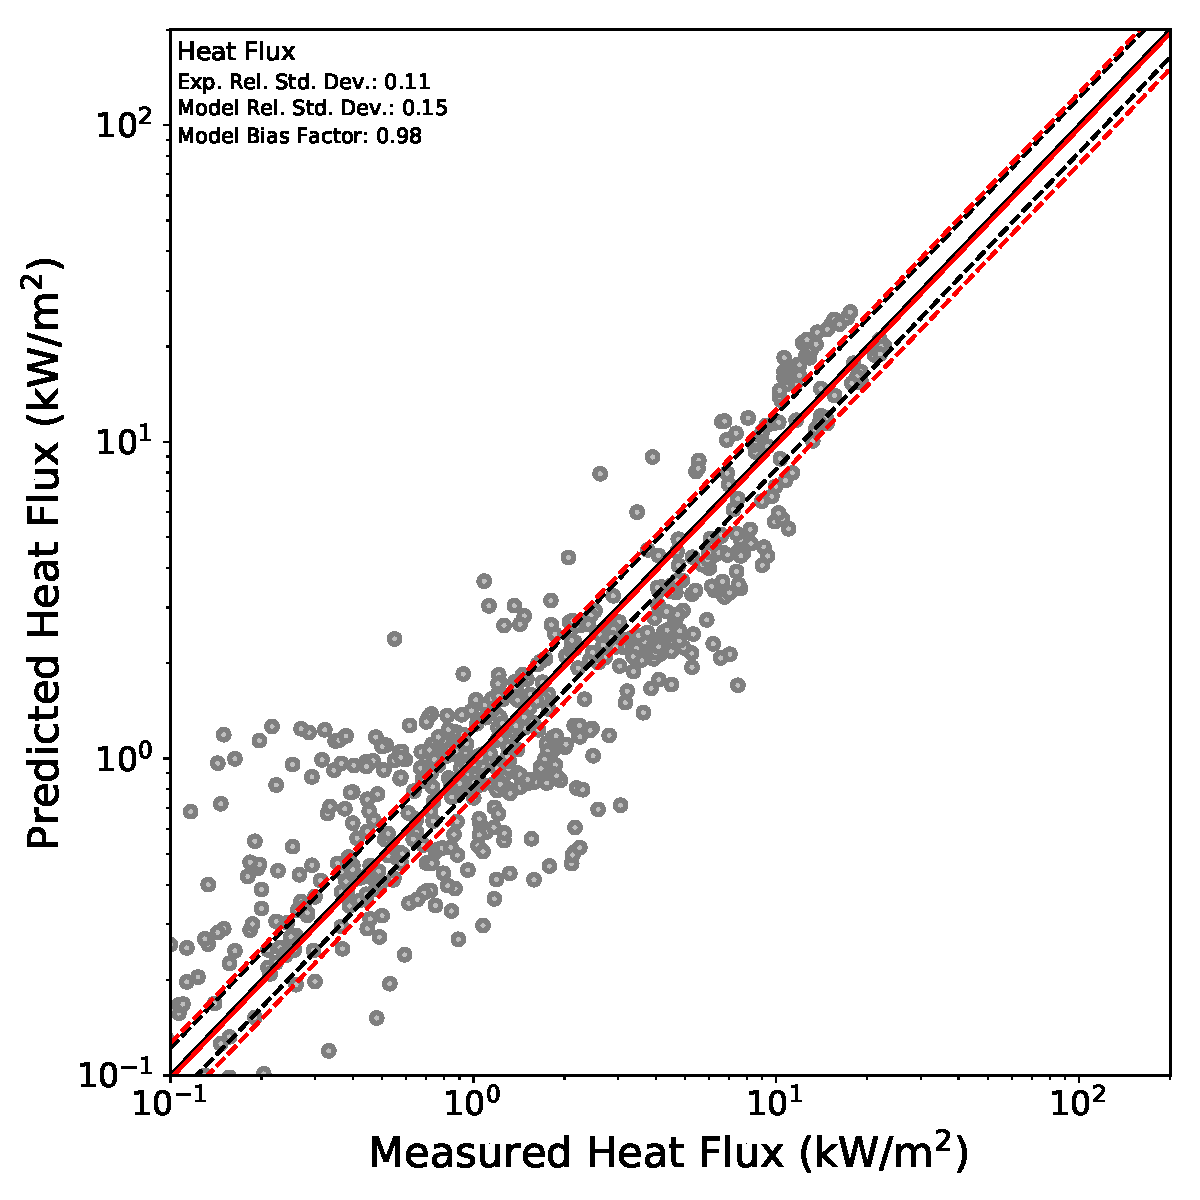
\includegraphics[width=\columnwidth]{../../Plots/Validation/Heat_Flux/loglog_HFs}
	\caption{Summary of measured and predicted heat flux measurements.}
	\label{fig:loglog_HFs}
\end{figure}

\clearpage
\subsection{Summary}
Table~\ref{table:stats_compare} compares the model bias factor ($\delta$), the experimental relative standard deviation ($\sigma_E$), and model relative standard deviation ($\sigma_M$) for each data quantity discussed above calculated across all appropriate time durations of the burner experiments to the same values that are listed in FDS Validation Guide for the corresponding data type based on all data within the FDS validation database. 
\begin{table}[!ht]
\caption[Calculated $\delta$, $\sigma_E$, and $\sigma_M$ Values Compared to Values Stated in FDS Validation Guide.]{Comparison of Model Bias Factor ($\delta$) and Relative Standard Deviation of Experimental Data ($\sigma_E$) and Model Data ($\sigma_M$) from all Tests and Same Values Listed in FDS Validation Guide for Each Data Type.}
\begin{center}
\begin{tabular}{lcccccccc}
\toprule
					& & \multicolumn{3}{c}{\textbf{\underline{Calculated}}} & & \multicolumn{3}{c}{\textbf{\underline{FDS Validation}}}   \\
\textbf{Quantity} 	& & \multicolumn{3}{c}{\textbf{\underline{Values}}} 	& & \multicolumn{3}{c}{\textbf{\underline{Guide}}} \\
				 	& & $\delta$ 	&  $\sigma_E$ 	& 	$\sigma_M$ 			& & $\delta$ 	&  $\sigma_E$ 	& 	$\sigma_M$ 		\\	
\midrule
Hot Gas Layer 		& & \multirow{2}{*}{0.97} & \multirow{2}{*}{0.05} & \multirow{2}{*}{0.05} & & \multirow{2}{*}{1.04} & \multirow{2}{*}{0.07} & \multirow{2}{*}{0.07} 	\\
Temperature 		& &					   	  & 					  & 					  & &						& 					   &						\\
\multicolumn{9}{c}{} \\
Ceiling Jet 		& & \multirow{2}{*}{1.03} & \multirow{2}{*}{0.06} & \multirow{2}{*}{0.06} & & \multirow{2}{*}{1.04} & \multirow{2}{*}{0.07} & \multirow{2}{*}{0.13} 	\\
Temperature 		& & 					  & 					  & 					  & &						& 					   &						\\
\multicolumn{9}{c}{} \\
Oxygen 				& & \multirow{2}{*}{1.08}  & \multirow{2}{*}{0.08} & \multirow{2}{*}{0.15} & & \multirow{2}{*}{0.99} & \multirow{2}{*}{0.08} & \multirow{2}{*}{0.14} 	\\
Concentration 		& & 					   & 					  & 					   & & 						& 					   &						\\
\multicolumn{9}{c}{} \\
Carbon Dioxide 		& & \multirow{2}{*}{0.96}  & \multirow{2}{*}{0.08} & \multirow{2}{*}{0.14} & & \multirow{2}{*}{1.00} & \multirow{2}{*}{0.08} & \multirow{2}{*}{0.12} 	\\
Concentration 		& & 					   & 					  & 					   & & 						& 					   &						\\
\multicolumn{9}{c}{} \\
Gas Velocity 		& & 1.05  & 0.06 & 0.26 & & 0.99 & 0.08 & 0.09 	\\
\multicolumn{9}{c}{} \\
Heat Flux 			& & 0.98  & 0.11 & 0.15 & & 0.98 & 0.11 & 0.24 	\\
\bottomrule
\end{tabular}
\end{center}
\label{table:stats_compare}
\end{table}

Overall, the agreement between the FDS simulation data and experimental data for the gas burner experiments is consistent with the statistical values given by the FDS Validation Guide. For the hot gas layer temperature, ceiling jet temperature, and heat flux, the model bias calculated for the gas burner simulations is equal to or better than (closer to the ideal value of 1) the overall model bias values given by the FDS Validation Guide. Additionally, the relative standard deviations of the experimental data and model data for these three quantities are equal to or less than (better than) the corresponding values for the same data types listed in the validation guide. 

The $\delta$, $\sigma_E$, and $\sigma_M$ values produced by the gas burner model and experimental data for both the $O_2$ and $CO_2$ gas concentrations were very close to the values documented in the FDS Validation Guide. The $\sigma_E$ values are equal in both comparisons and the $\sigma_M$ values are greater in magnitude by only 0.01 and 0.02 compared to the validation guide values for oxygen and carbon dioxide concentration, respectively. Finally, based on the data from gas burner simulations, the oxygen concentration model bias is worse (further from the ideal value of 1) by 7~\% and carbon dioxide concentration model bias is worse by 4~\% compared to the documented values in the FDS Validation Guide.

The most significant discrepancy between the documented values and values from the gas burner models is seen in the gas velocity comparison, in which $\sigma_M$ was calculated as being greater than the $\sigma_M$ from the validation guide by a value 0.18. This discrepancy may exist for a few of reasons. First, gas velocity was one of the quantities with the highest uncertainty associated with the experimental measurements. Also, as previously mentioned, the experiments were conducted outdoors, so environmental conditions may have affected the measurements, even though only data from BDPs that were fully inside the structures were considered. Almost all ([CHECK VALIDATION GUIDE FOR EXACT NUMBER]) the tests used to calculate the $\delta$, $\sigma_E$, and $\sigma_M$ within the validation guide were conducted in a laboratory setting, which could explain the significantly smaller model relative standard deviation. Finally, due to the nature of the fire environment at the time of the measurements, it's possible that turbulent flow was occurring through the vents (especially the roof vent in Tests~5 and 6) at the time of the measurements. LES CFD models, like FDS, tend to be limited more in terms of accurately measuring turbulent flow than compared to measurements during other conditions.
